\subsection{Rainfall}

In this subsection, we will analyze the rainfall through three perspectives: the rainfall pattern and spatial distribution; the mean and distribution of rain volume; and the extreme values.

\subsubsection{Pattern and spatial rainfall distribution}

Following the workflow proposed in the Metrics section, we can quantify the spatial distribution of rainfall using the ETS and Pearson correlation coefficient. This analysis focuses on a specific area (106-51°W, 10-41°N) over a six-day forecast period, from July 3rd to July 9th (00 UTC). Upon reviewing the literature \cite{marchok2007validation}, \cite{brackins2020evaluation}, \cite{luitel2018verification}, we found that these metrics are influenced by the forecasted track and are typically calculated over a defined region, usually a 500-600 km radius around the best track trajectory, rather than the broader area we are examining. In their 2007 study, Marchok et al. discuss this in detail and suggest potential improvements to compute those metrics, also regarding resolution dependencies. We opted to calculate the accumulated area to reduce the track error effect, though it is important to note that this approach may also capture local rainfall accumulations. In our study area, identifying the hurricane is relatively straightforward; for example, reports indicate that Beryl produced 13.2 inches (approximately 335 mm) of accumulated rainfall over Jamaica \cite{li2025generative}, so because of this, the broader area should not be this much of a problem, but meant to be a simple view of the spatial rainfall distribution. For future work, we propose adapting the previous approach to more accurately represent both the ETS and Pearson correlation coefficients.

Figure \ref{fig:threatscore} illustrates the ETS for various rainfall thresholds (in mm). These thresholds were determined using a log distribution, similar to the method presented by Marchok et al. in 2007. The maximum threshold was established with consideration of the maximum distribution observed in the datasets \footnote{The Python function used was: \texttt{numpy.logspace(numpy.log10(0.01), numpy.log10(350), num=12)}}. For instance, the maximum accumulated rainfall measured was 252.5 mm, 252.0 mm, 453.7 mm, 485.4 mm, 359.6 mm for GPM-IMERG, ERA5, GSMaP, CP-ON, CP-OFF, respectively.

\begin{figure}[!ht]
	\centering
	\caption{Equitable Threat Score for all experiments, ERA5 dataset and GSMaP dataset.} % Título acima da figura
	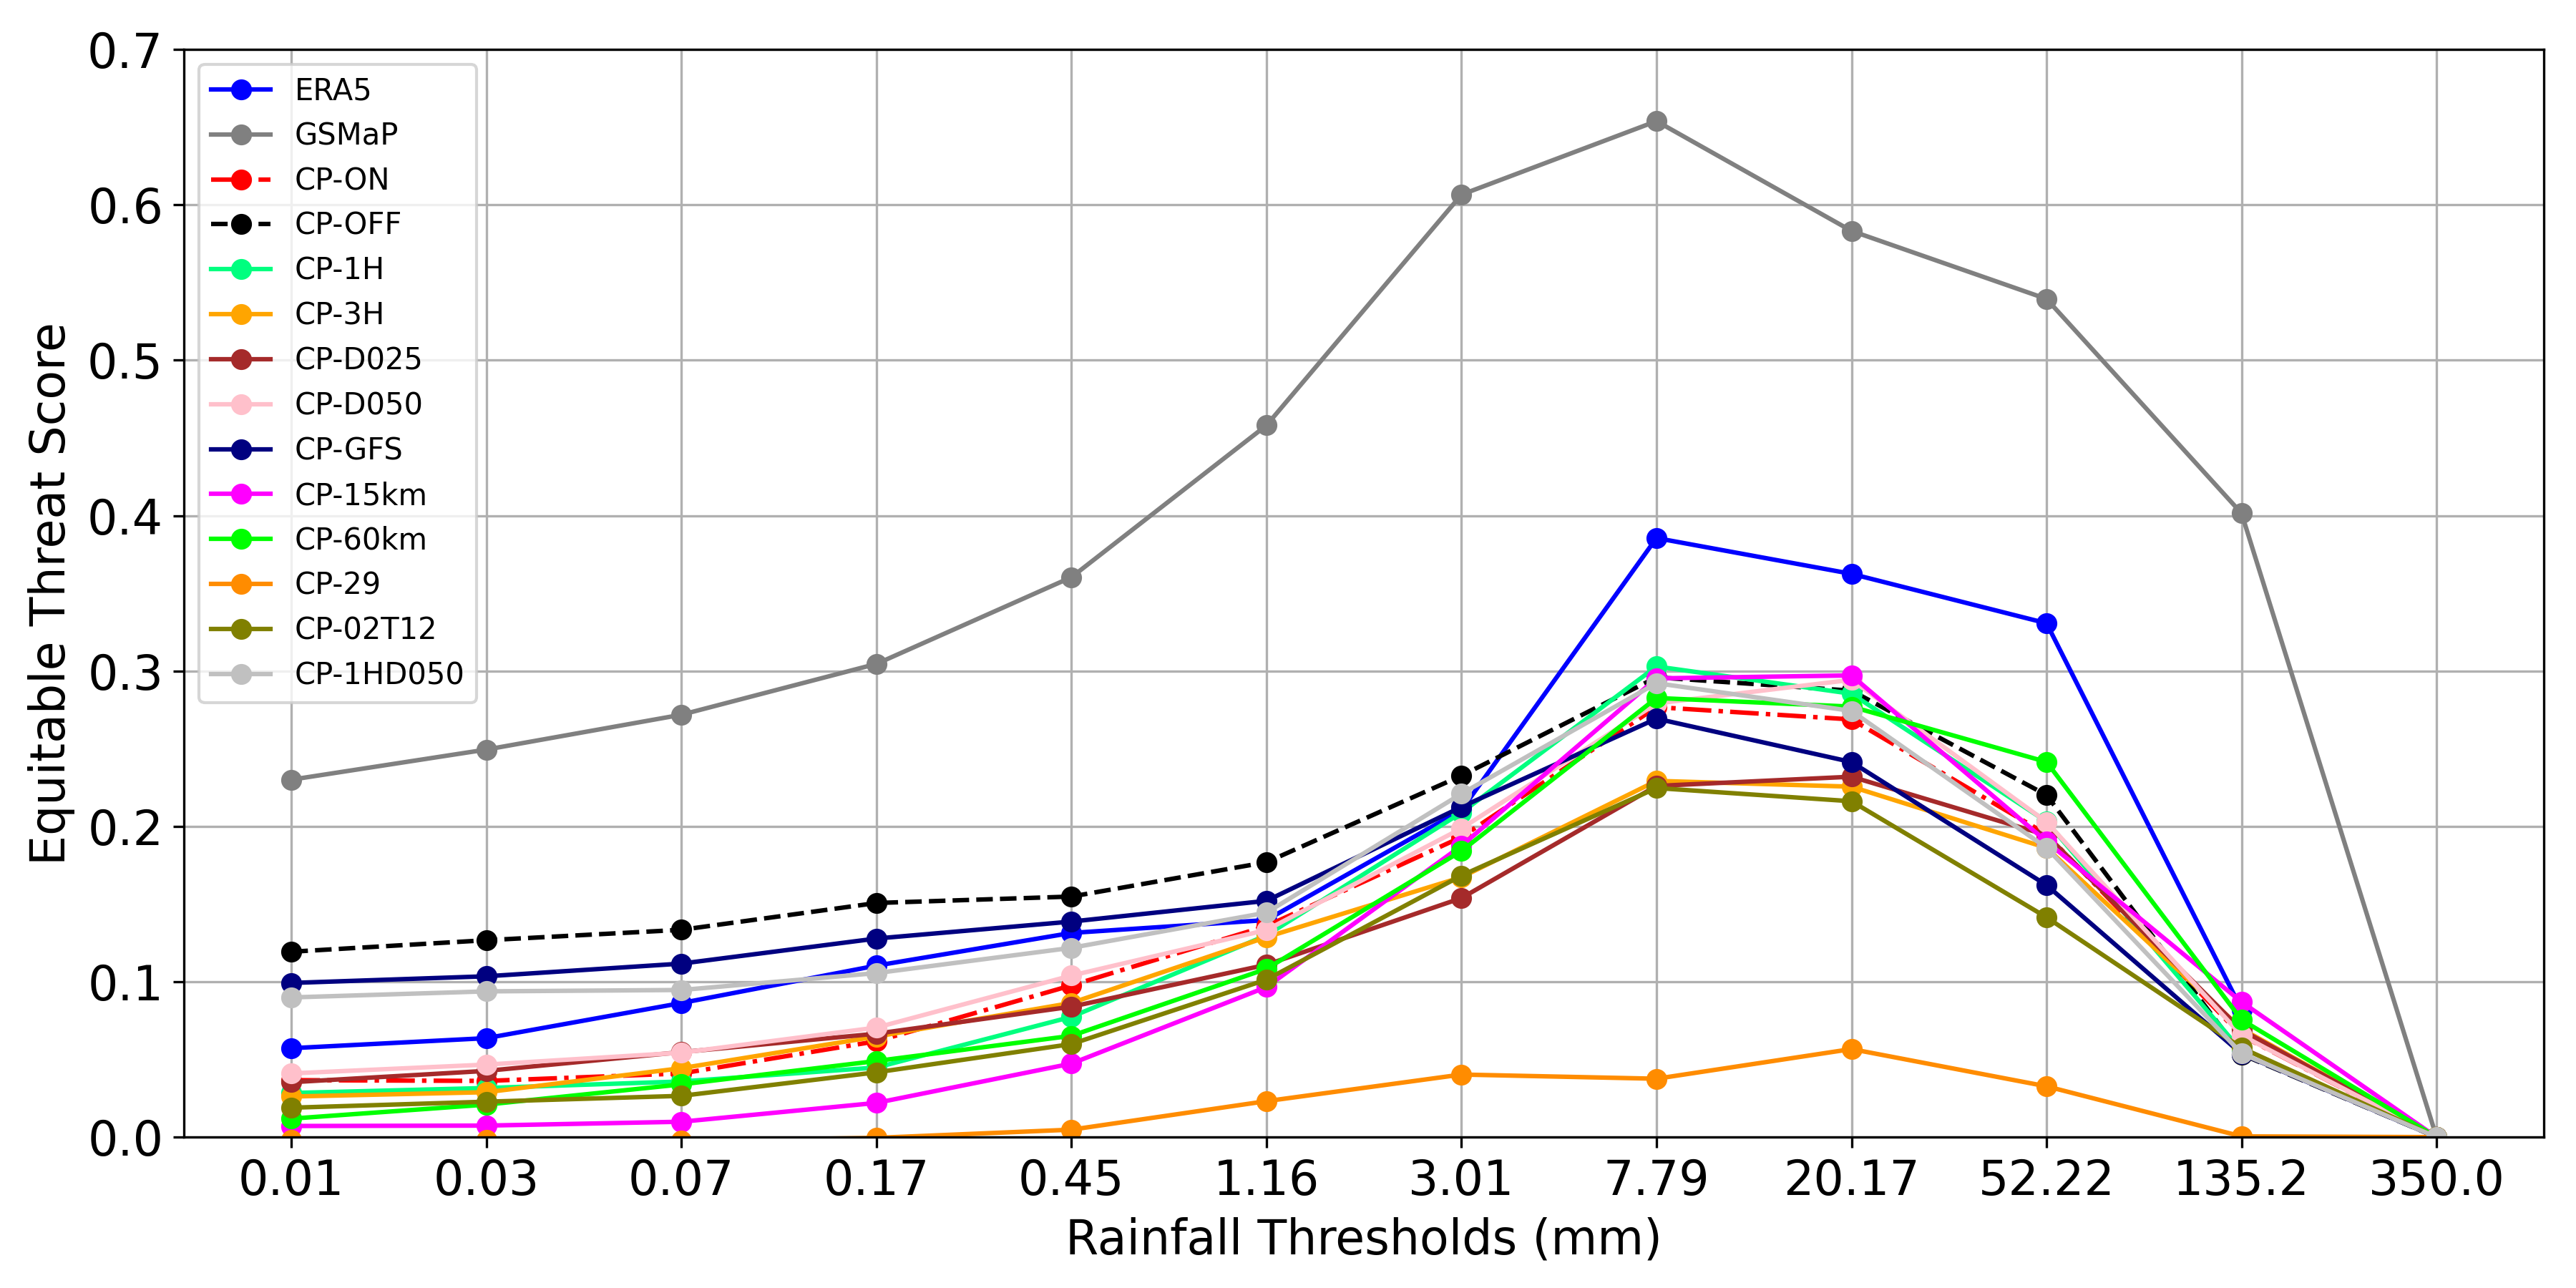
\includegraphics[width=\textwidth]{docs/figuras/chapter5/ets_all_experiments_logx_FINAL.png} 
	\vspace{0.5em}
	Source: Made by the author (2025).  % Fonte abaixo da imagem
	\label{fig:threatscore} % Label para referenciar no texto
\end{figure}

The GSMaP exhibits the best score due to its nature as a satellite-based system. It is important to highlight that for this and other analyses, both GSMaP, ERA5, and GPM-IMERG data were downscaled to the model's resolution of 30 km. In the case of GSMaP, the resolution was reduced from 4 km to 30 km. The further analysis will explicitly mention this whenever the data is not downscaled.

ERA5 shows better agreement in the moderate to extreme rainfall range (between 3 and 135 mm), but it is important to note that the maximum rainfall is relatively low compared to GPM-IMERG. Thus, ERA5 does not score well regarding rainfall data produced by this event.

In general, the forecasts from MONAN display similar behavior, with some outliers. For example, CP-OFF shows a better score at the lower thresholds compared to other forecasts, meaning that local rainfall is slightly better in agreement with the observed data, but it displays the same trend in the extreme thresholds. Another outlier is CP-29, which exhibits poor agreement with the observed data, especially due to a poor predicted trajectory.

At more extreme thresholds (above 135 mm), the scores for all data types drop significantly, indicating the need for further investigation into this topic.

The Pearson correlation coefficient is shown next, in Figure XXX. This coefficient was calculated across the entirety of the spatial domain, indicating that it provides a correlation value representative of the entire scene.

\begin{figure}[!ht]
	\centering
	\caption{Spatially averaged Pearson correlation coefficient over the entire domain} % Título acima da figura
	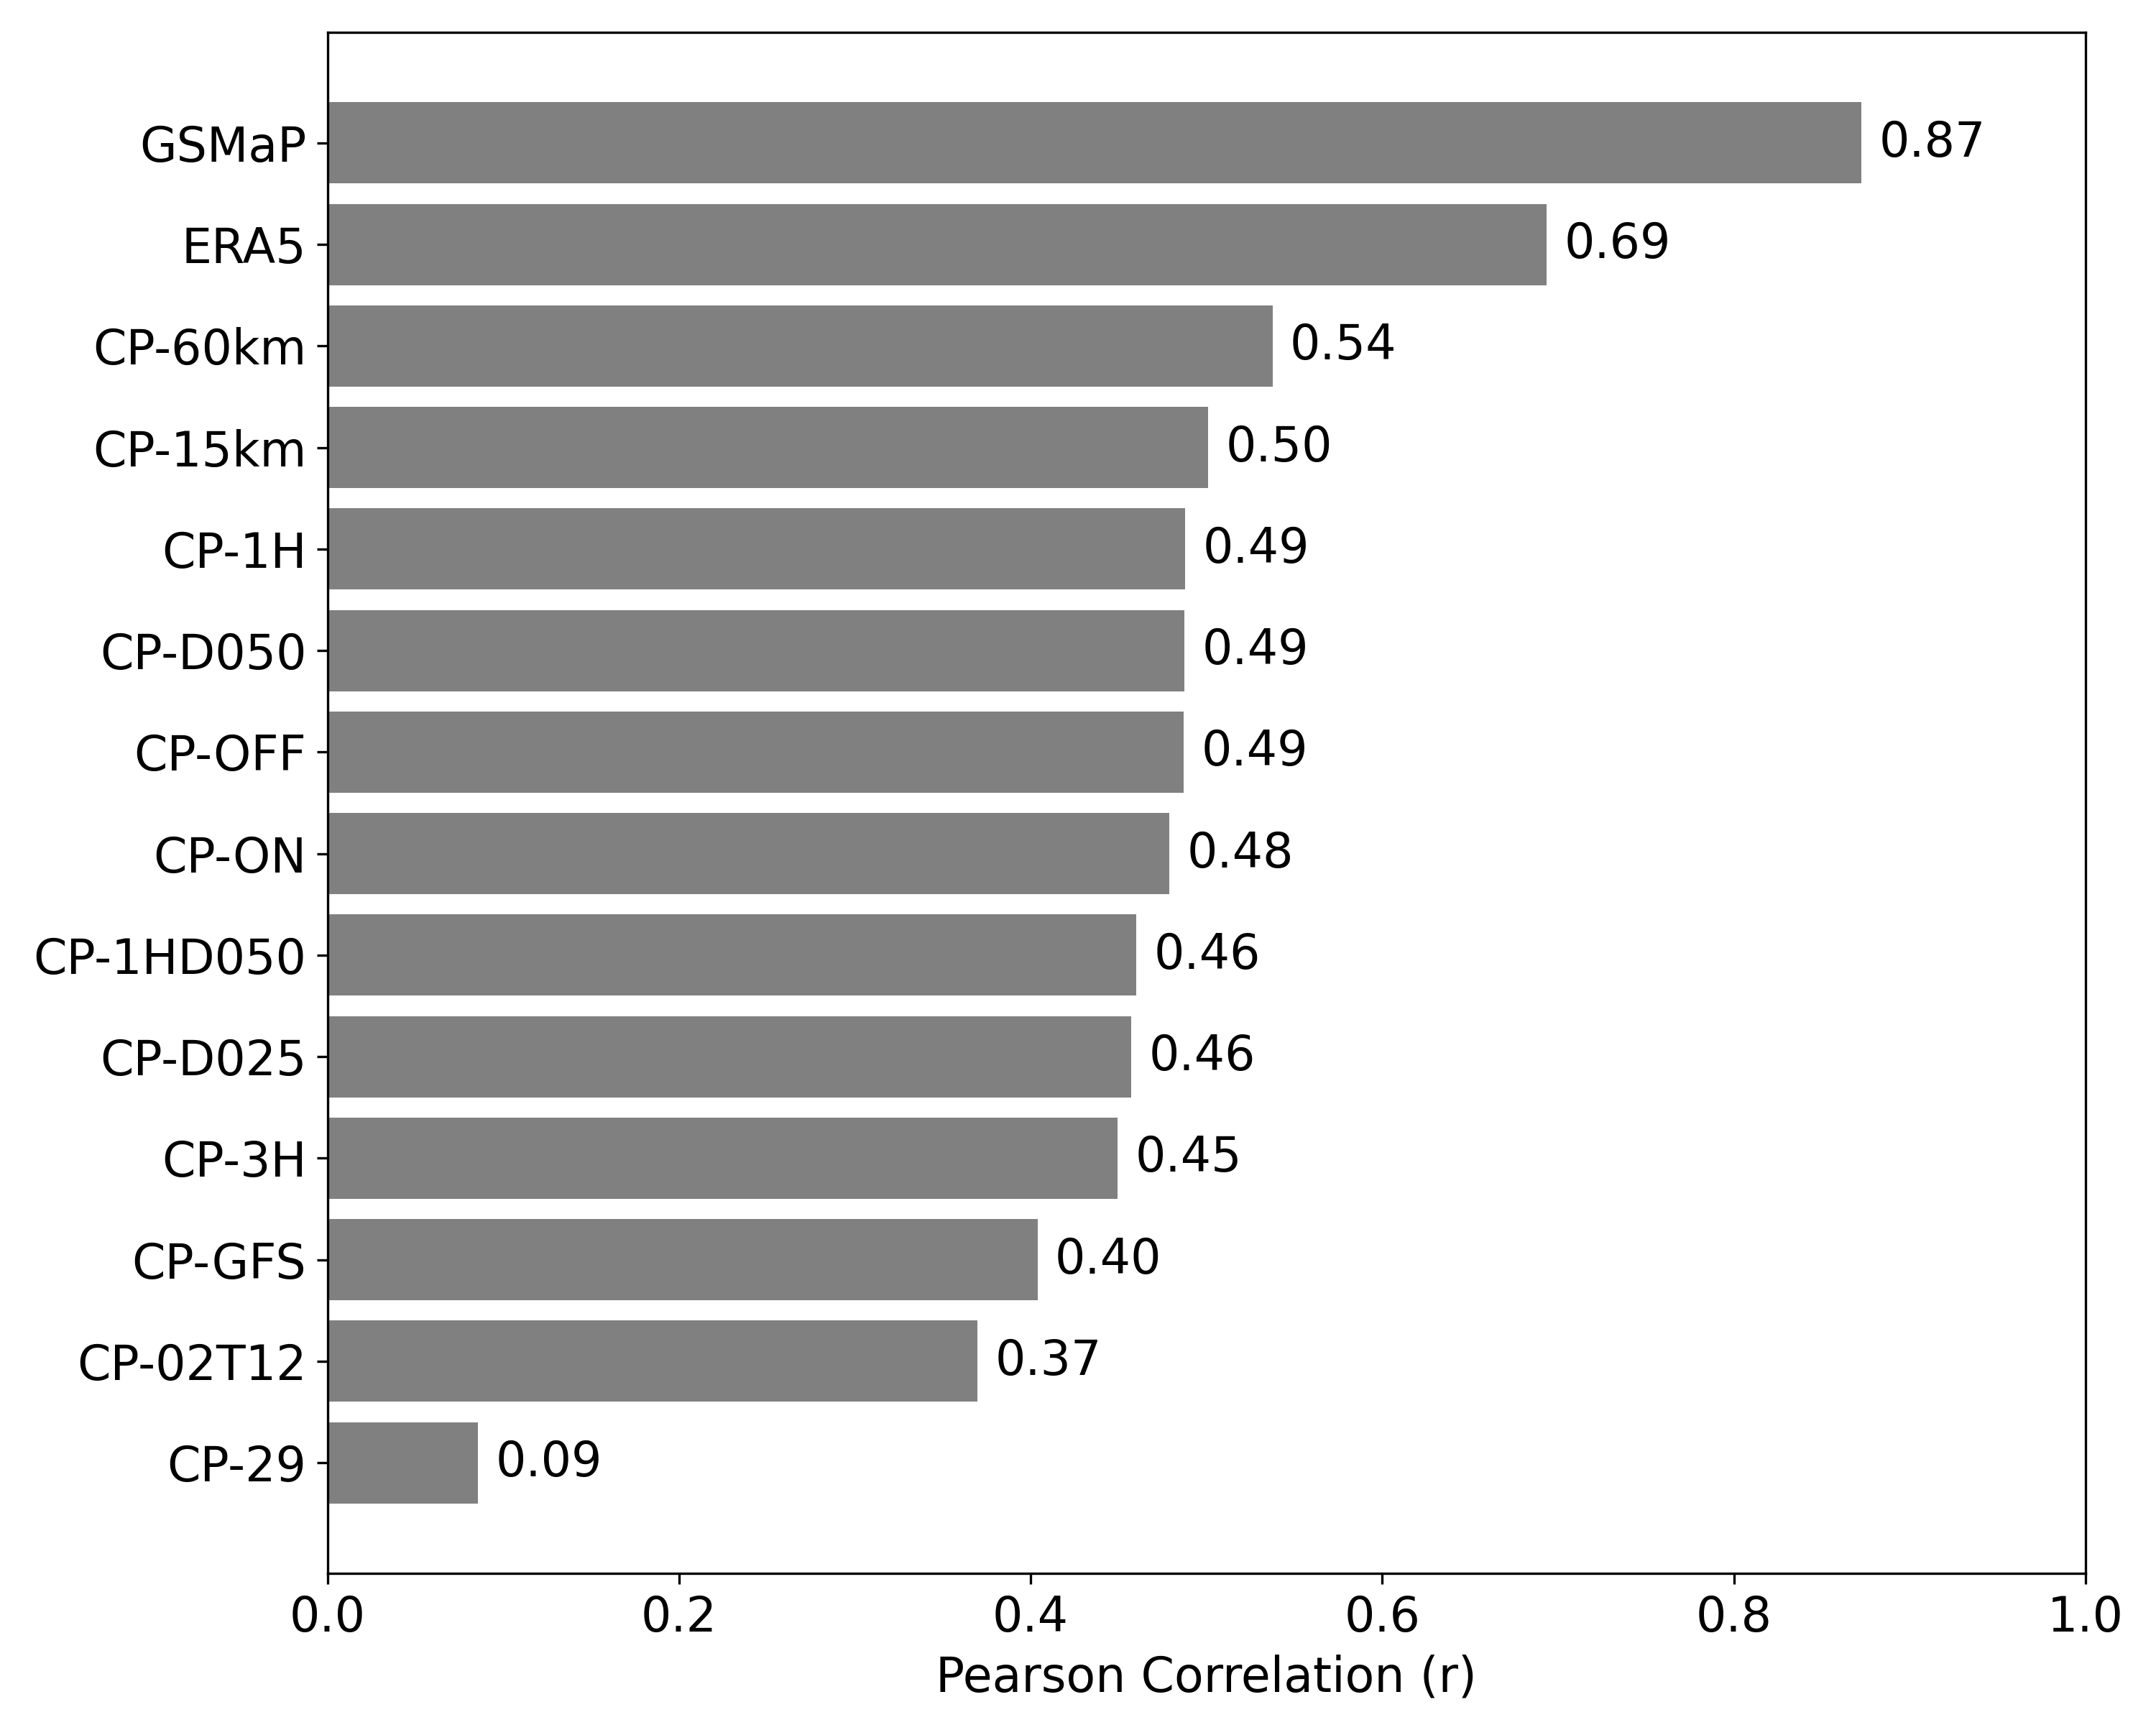
\includegraphics[width=\textwidth]{docs/figuras/chapter5/pearson_correlation_bar_chart_FINAL.png} 
	\vspace{0.5em}
	Source: Made by the author (2025).  % Fonte abaixo da imagem
	\label{fig:pearson} % Label para referenciar no texto
\end{figure}

Once again, the data from GSMaP and ERA5 stand out with the strongest correlations with GPM-IMERG. Interestingly, this highlights the effects that changes in resolution can have, as seen more clearly in the panel of Figure \ref{fig:dpearson}.

Regarding the forecasts from MONAN, the average correlation is around moderate, excluding outliers such as GFS, CP-29, and CP-02T12. Note that for the last two forecasts, the bias from the trajectory itself strongly influences the calculation of this metric, as CP-29 and CP-02T12 also had the largest tracking errors (Figure \ref{fig:trackerrors}).

To better infer the locations with the best/worst correlations, as well as to gain a clearer understanding of the temporal evolution of correlation in the forecasts, Figure \ref{fig:dpearson} displays the correlation spatially, computed from daily rainfall accumulations.

\begin{figure}[!ht]
	\centering
	\caption{Spatial distribution of daily Pearson correlation values to assess temporal evolution of forecast performance} % Título acima da figura
	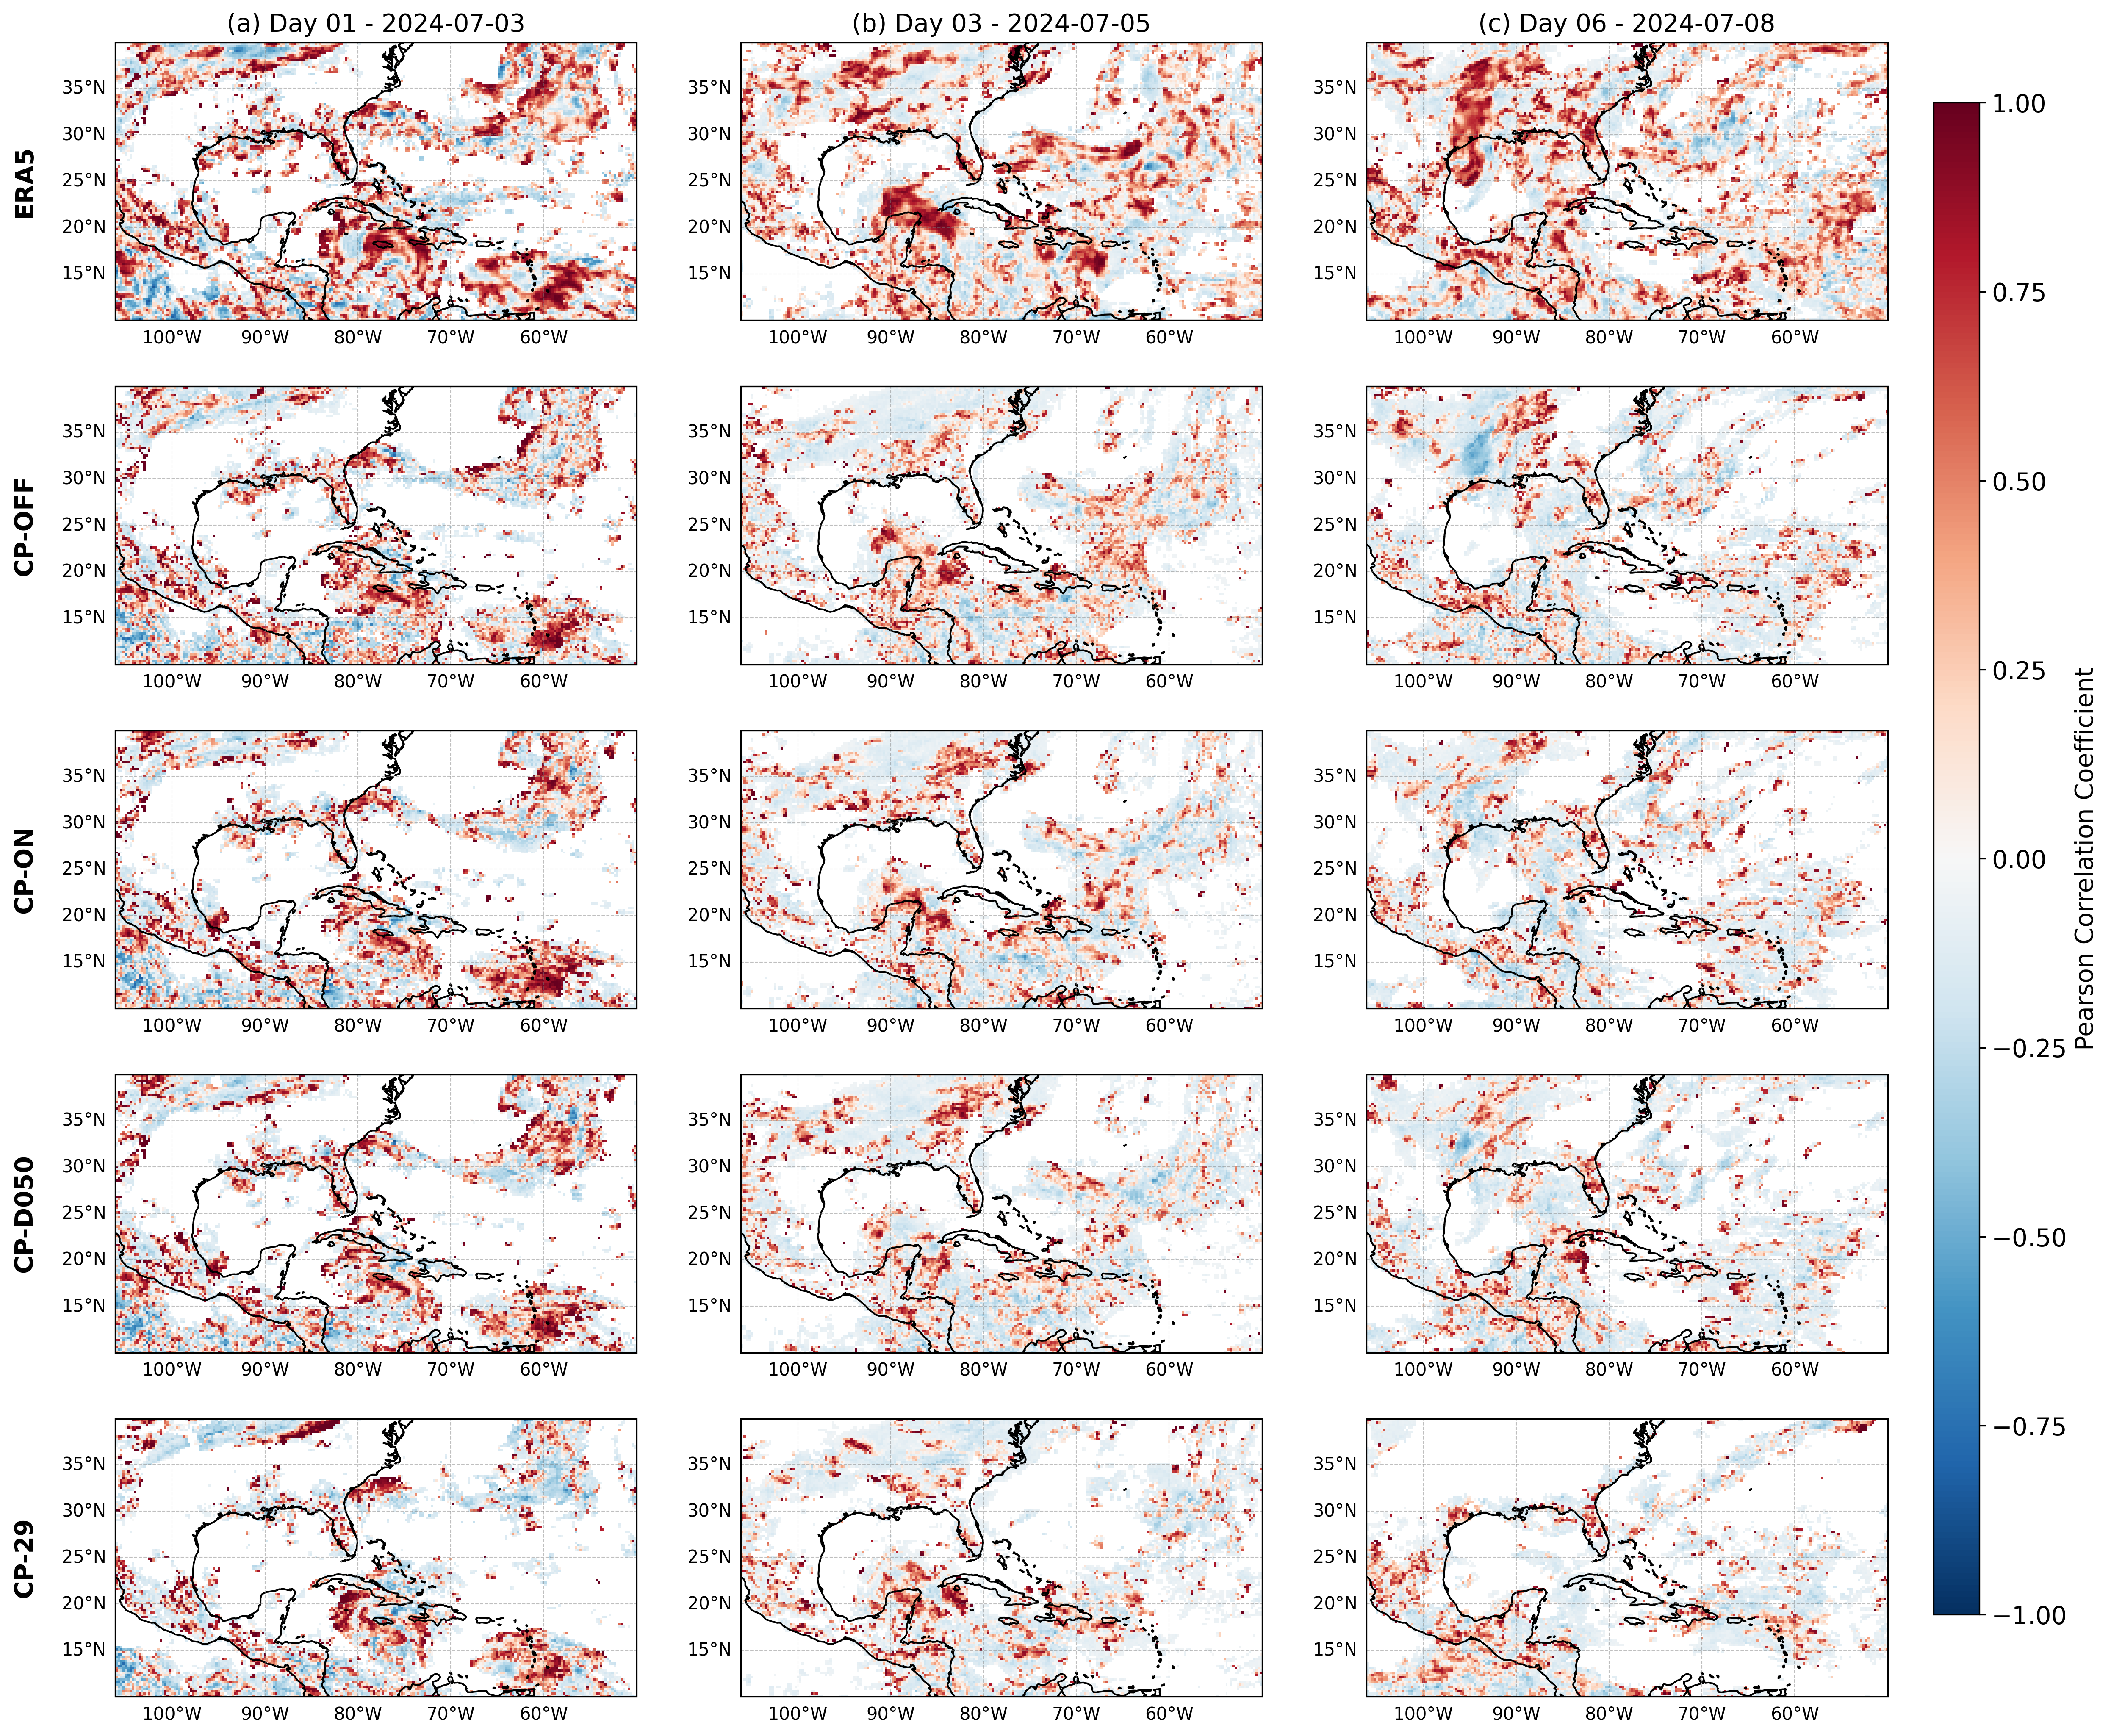
\includegraphics[width=\textwidth]{docs/figuras/chapter5/painel_correlation_selected_experiments_days_nomeado.png} 
	\vspace{0.5em}
	Source: Made by the author (2025).  % Fonte abaixo da imagem
	\label{fig:dpearson} % Label para referenciar no texto
\end{figure}

In this figure, the selected days represent: (a) the starting point of forecasts, immediately following the weakening of Hurricane Beryl, but corresponding to the highest observed rainfall (over Jamaica); (b) its passage over the Yucatán Peninsula, during which the hurricane weakens from Category 1 to a tropical storm; and (c) landfall in Texas on the North American continent. It is important to note that each column represents the accumulated rainfall for 24 hours; thus, panel (a) corresponds to rainfall accumulated over July 3rd, and so on.

The top row presents correlation values derived from ERA5 reanalysis, which exhibited strong correlations, while the bottom row shows the correlation from the CP-29 forecast, which had the weakest agreement. To evaluate the effect of cold pool parameterization, CP-ON and CP-OFF are aligned for comparison. Additionally, CP-D050 was selected as an example of moderate correlation to identify where the internal parameterization settings are influencing correlation variability. Other experiments referenced in the study are presented in the appendix.

Regarding the temporal evolution of correlation, a general degradation in forecast performance over time is observed, with the reanalysis data maintaining higher consistency, as expected. Notably, CP-29 shows a significantly sharper decline in correlation over time compared to CP-ON, for instance. 

For instance, CP-29 reveals a pronounced track error upon landfall in Texas (100–90°W, 25–35°N), as evidenced by a near-zero correlation in that region. In the same region, CP-D050 and CP-OFF present negative correlations when compared with CP-ON.

CP-D050 fails to represent rainfall over the Yucatán Peninsula, whereas CP-ON appears to generate more cohesive rainfall patterns than CP-OFF (20–25°N, 90–80°W). Both CP-D050, CP-ON, and CP-OFF also show localized overestimation of rainfall east of Cuba, a region that does show rainfall in the ERA5 dataset.

Selected snapshots corresponding to these dates were chosen to confirm the previously discussed relationships. A panel displaying these time steps alongside IMERG and GSMaP (both downscaled to 30 km resolution) is presented in Figure \ref{fig:snapshot}.

\begin{figure}[!ht]
	\centering
	\caption{Selected snapshots of rainfall fields from IMERG and GSMaP (30 km resolution) for key time steps} % Título acima da figura
	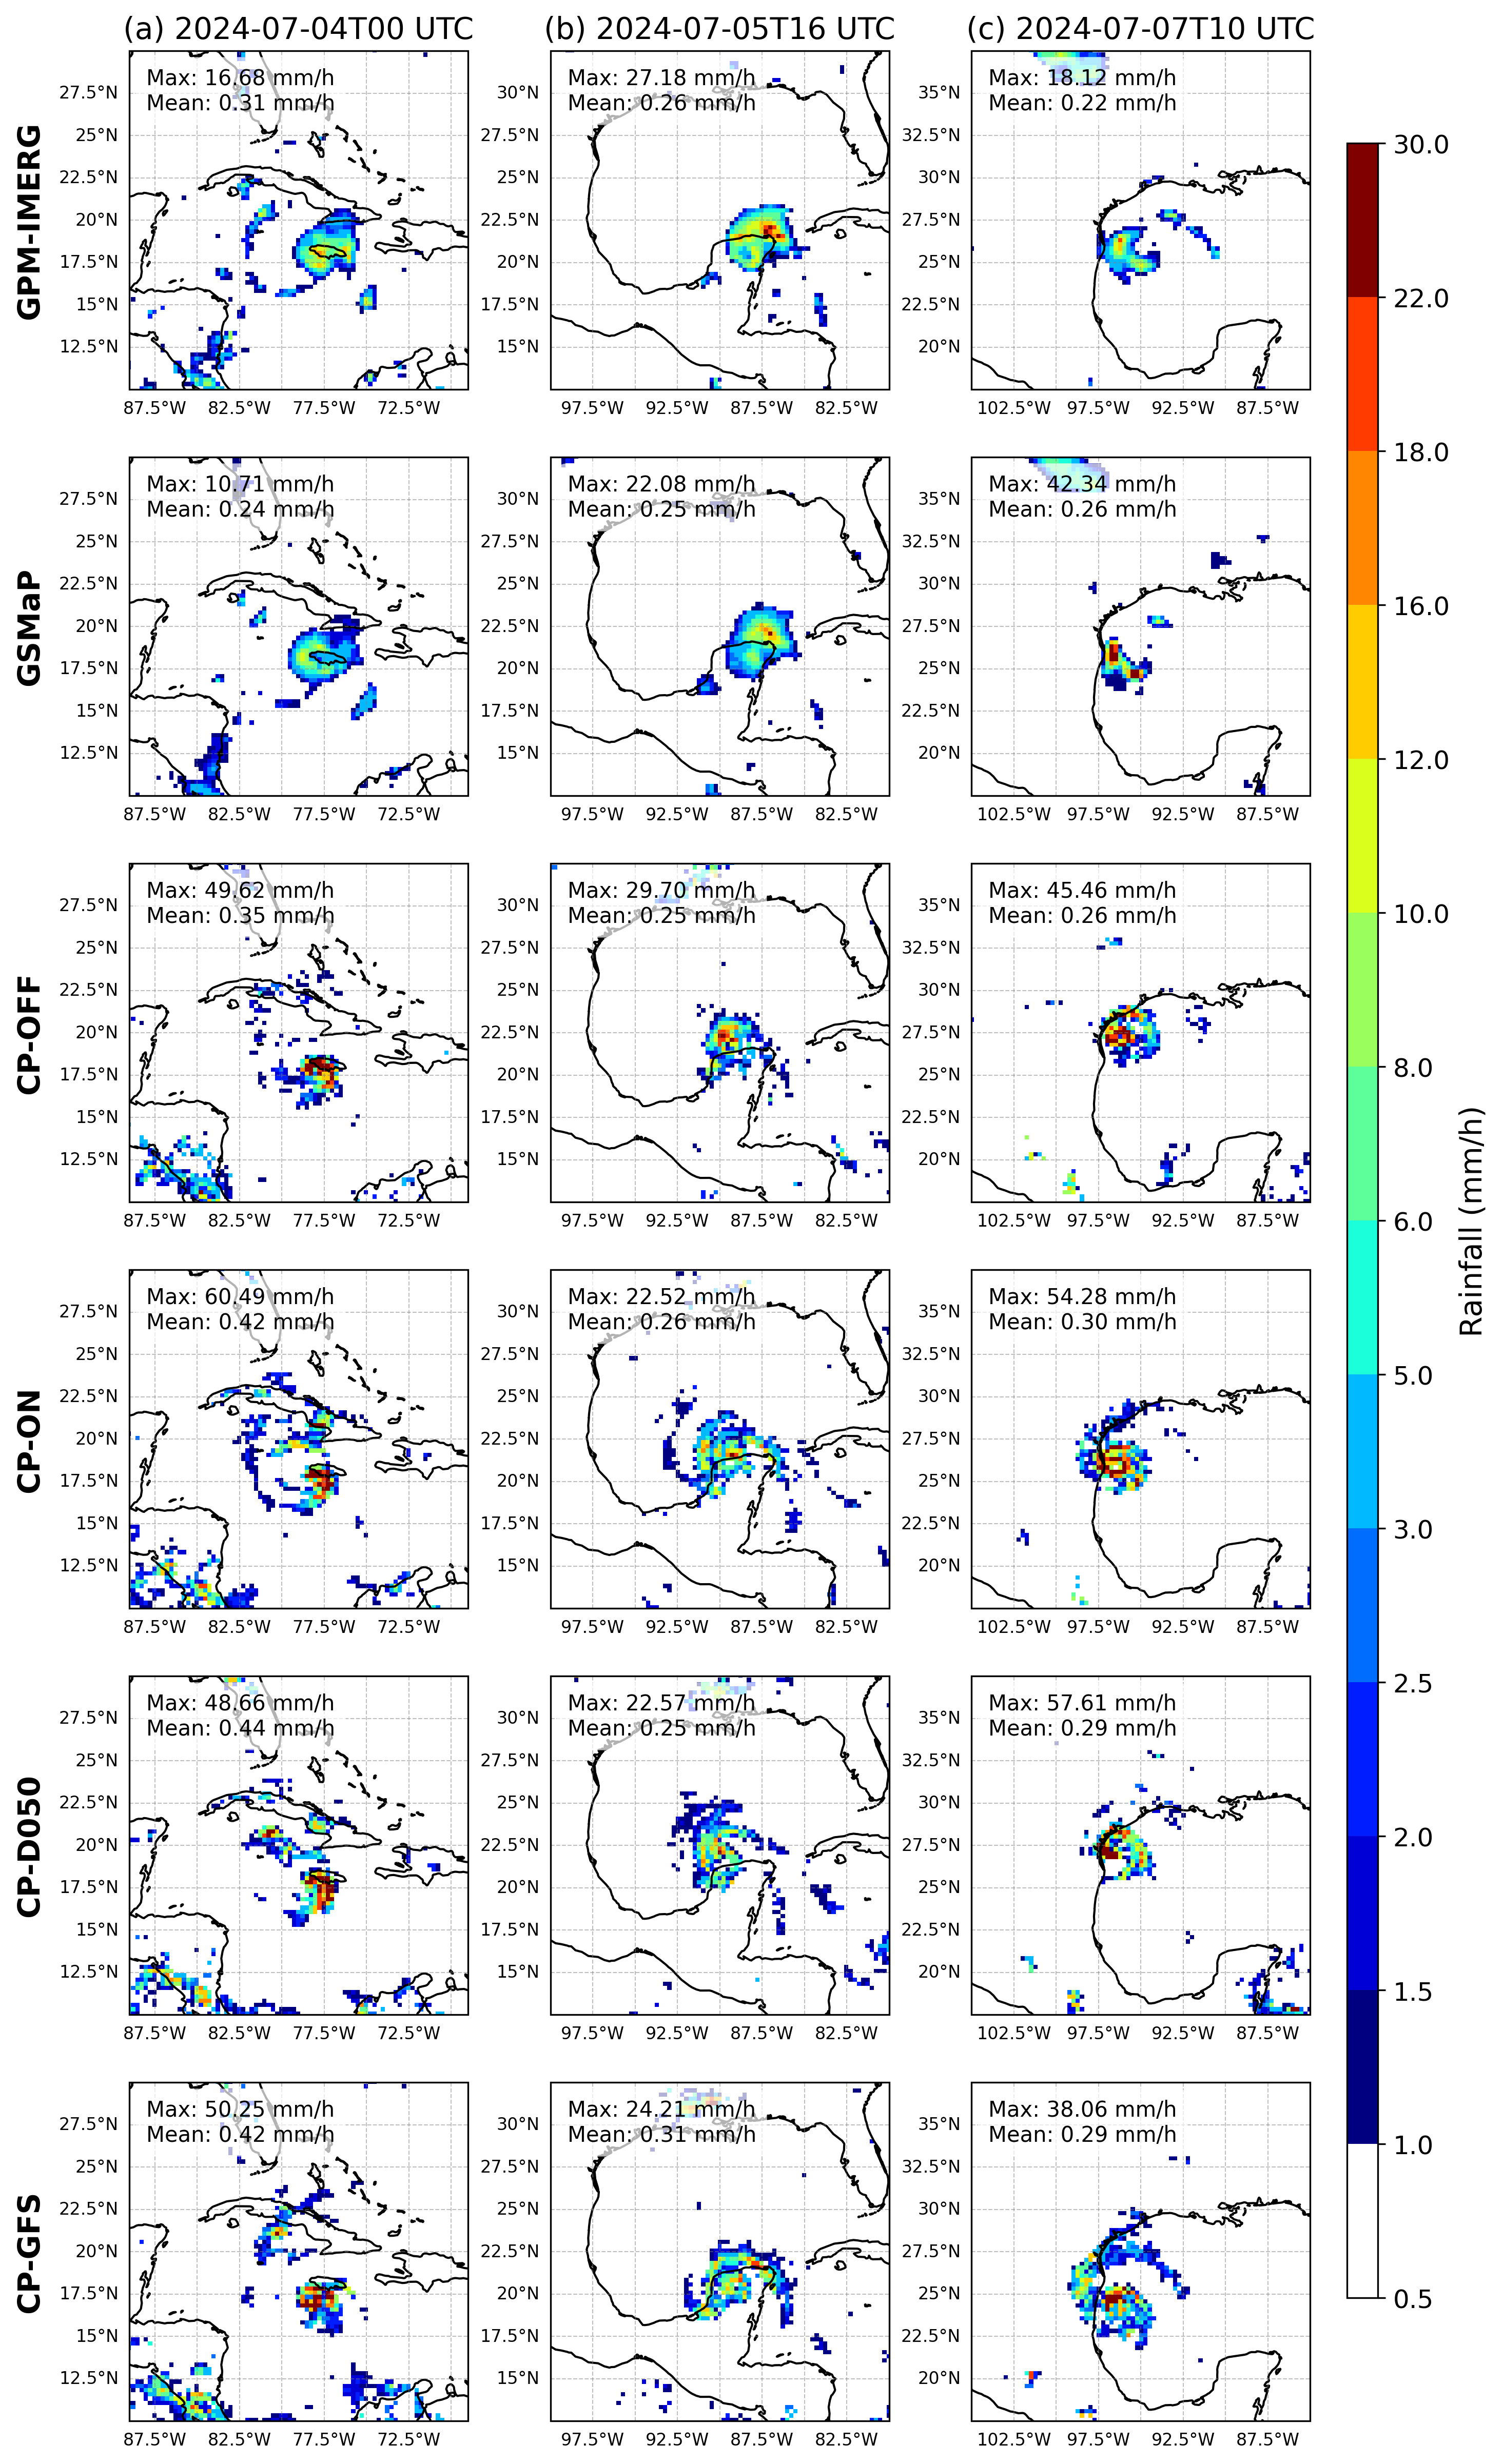
\includegraphics[width=\textwidth]{docs/figuras/chapter5/painel_instantaneous_rainfall_selected_with_stats_FINAL.png} 
	\vspace{0.5em}
	Source: Made by the author (2025).  % Fonte abaixo da imagem
	\label{fig:snapshot} % Label para referenciar no texto
\end{figure}

One of the most notable aspects across the panels is the skill of the parameterizations in generating cohesive rainfall patterns (e.g., CP-ON and CP-GFS in column a), and in some cases, reproducing the hurricane's spiral structure (panel b—seen in CP-ON, CP-D050, and CP-GFS).

Regarding maximum and average rainfall, the forecasts tend to overestimate precipitation relative to observations. However, in column (b), both CP-ON and CP-D050 are close to approximating the rainfall amounts observed by GSMaP.

It is evident that these panels visually reflect the patterns observed in the cross-track and along-track errors, particularly in column (c). For example, the Hurricane Beryl location by GPM-IMERG is slightly different from CP-ON, since the CP-ON forecast is located farther north.

The bias computed against GPM-IMERG is presented in Figure \ref{fig:biasgpm}. However, it is important to note that bias is not a particularly reliable metric for this type of phenomenon, as it is heavily influenced by trajectory errors inherent to tropical cyclone forecasts.

\begin{figure}[!ht]
	\centering
	\caption{Bias relative to GPM-IMERG for tropical cyclone rainfall forecasts} % Título acima da figura
	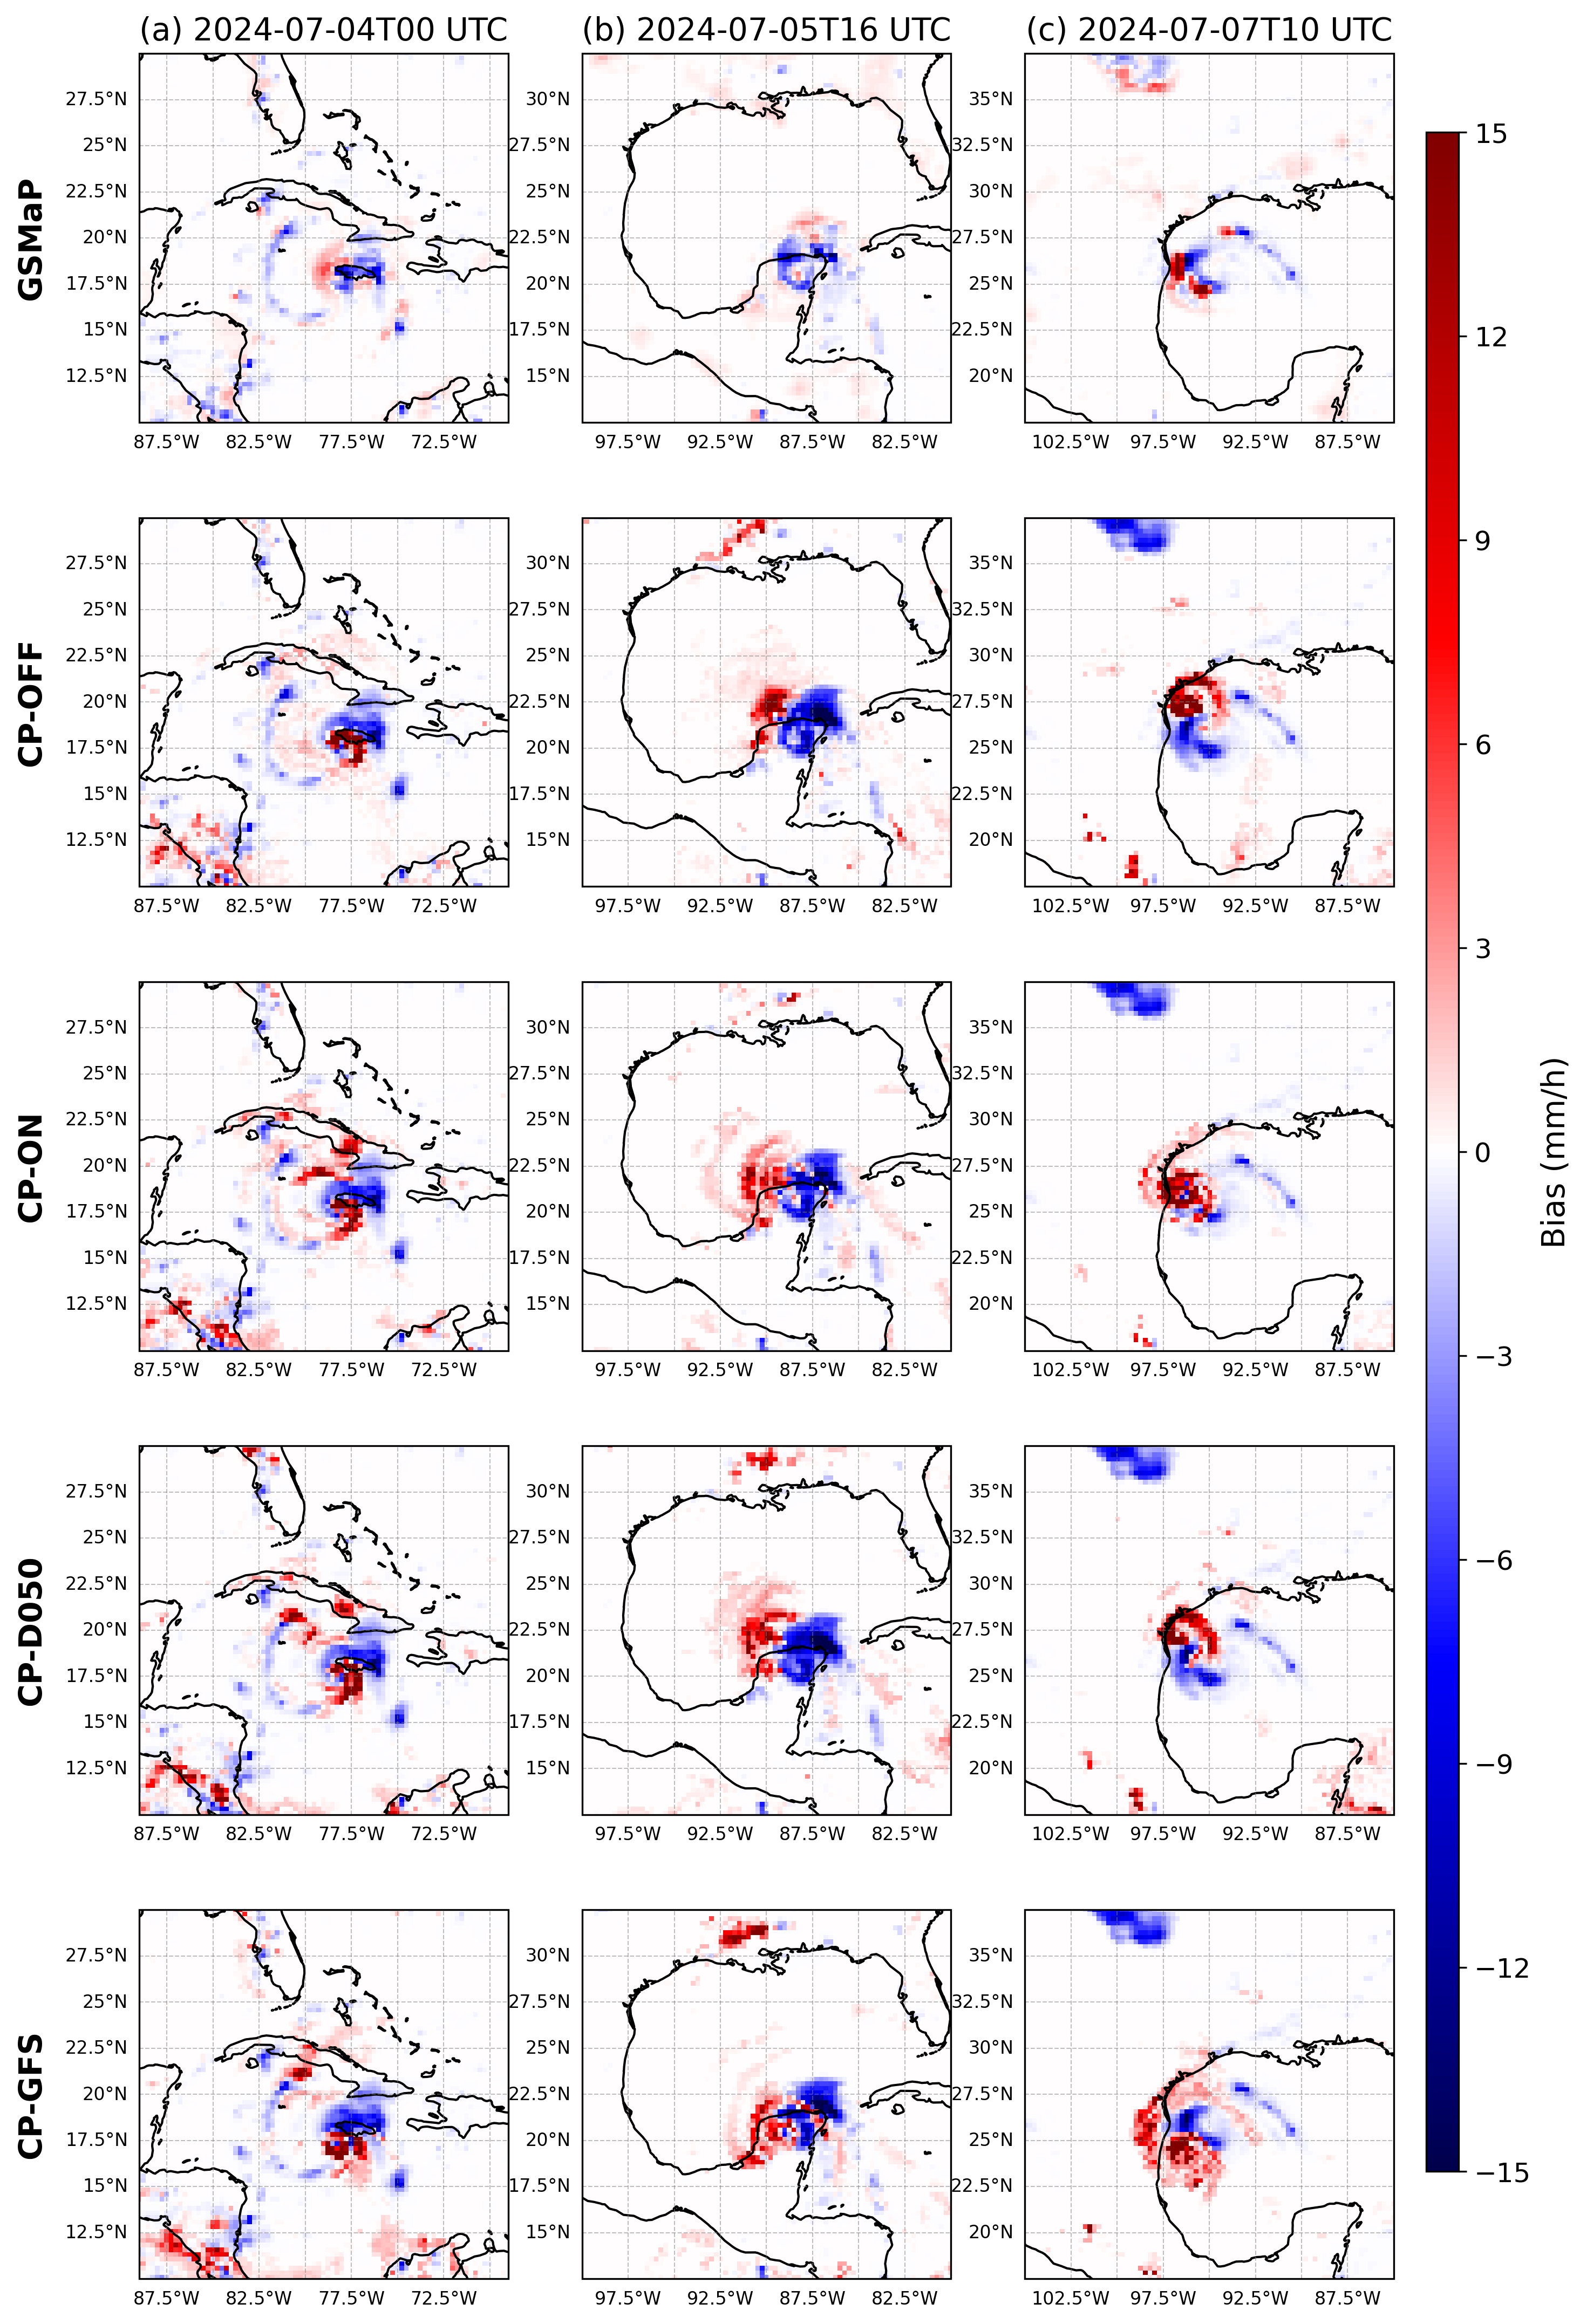
\includegraphics[width=\textwidth]{docs/figuras/chapter5/painel_bias_rainfall_selected_FINAL.png} 
	\vspace{0.5em}
	Source: Made by the author (2025).  % Fonte abaixo da imagem
	\label{fig:biasgpm} % Label para referenciar no texto
\end{figure}

Using the same example as before, in column (c), a positive bias can be observed in the hurricane region, clearly indicating that the hurricane position produced by CP-ON is farther north compared to GPM-IMERG. Moreover, this figure reinforces the results shown previously with the cross- and along-track errors (Figure \ref{fig:trackerrors}).

As previously discussed (Figures XXX and XXX), changing the horizontal resolution results in forecasts with good correlation. To further investigate this, Figure \ref{fig:biasgpm2} presents forecasts at 15 km, 30 km, and 60 km horizontal resolution, using the same spatial and temporal domains as in Figure \ref{fig:snapshot}.

\begin{figure}[!ht]
	\centering
	\caption{Spatial bias relative to GPM-IMERG, highlighting displacement effects in tropical cyclone forecasts} % Título acima da figura
	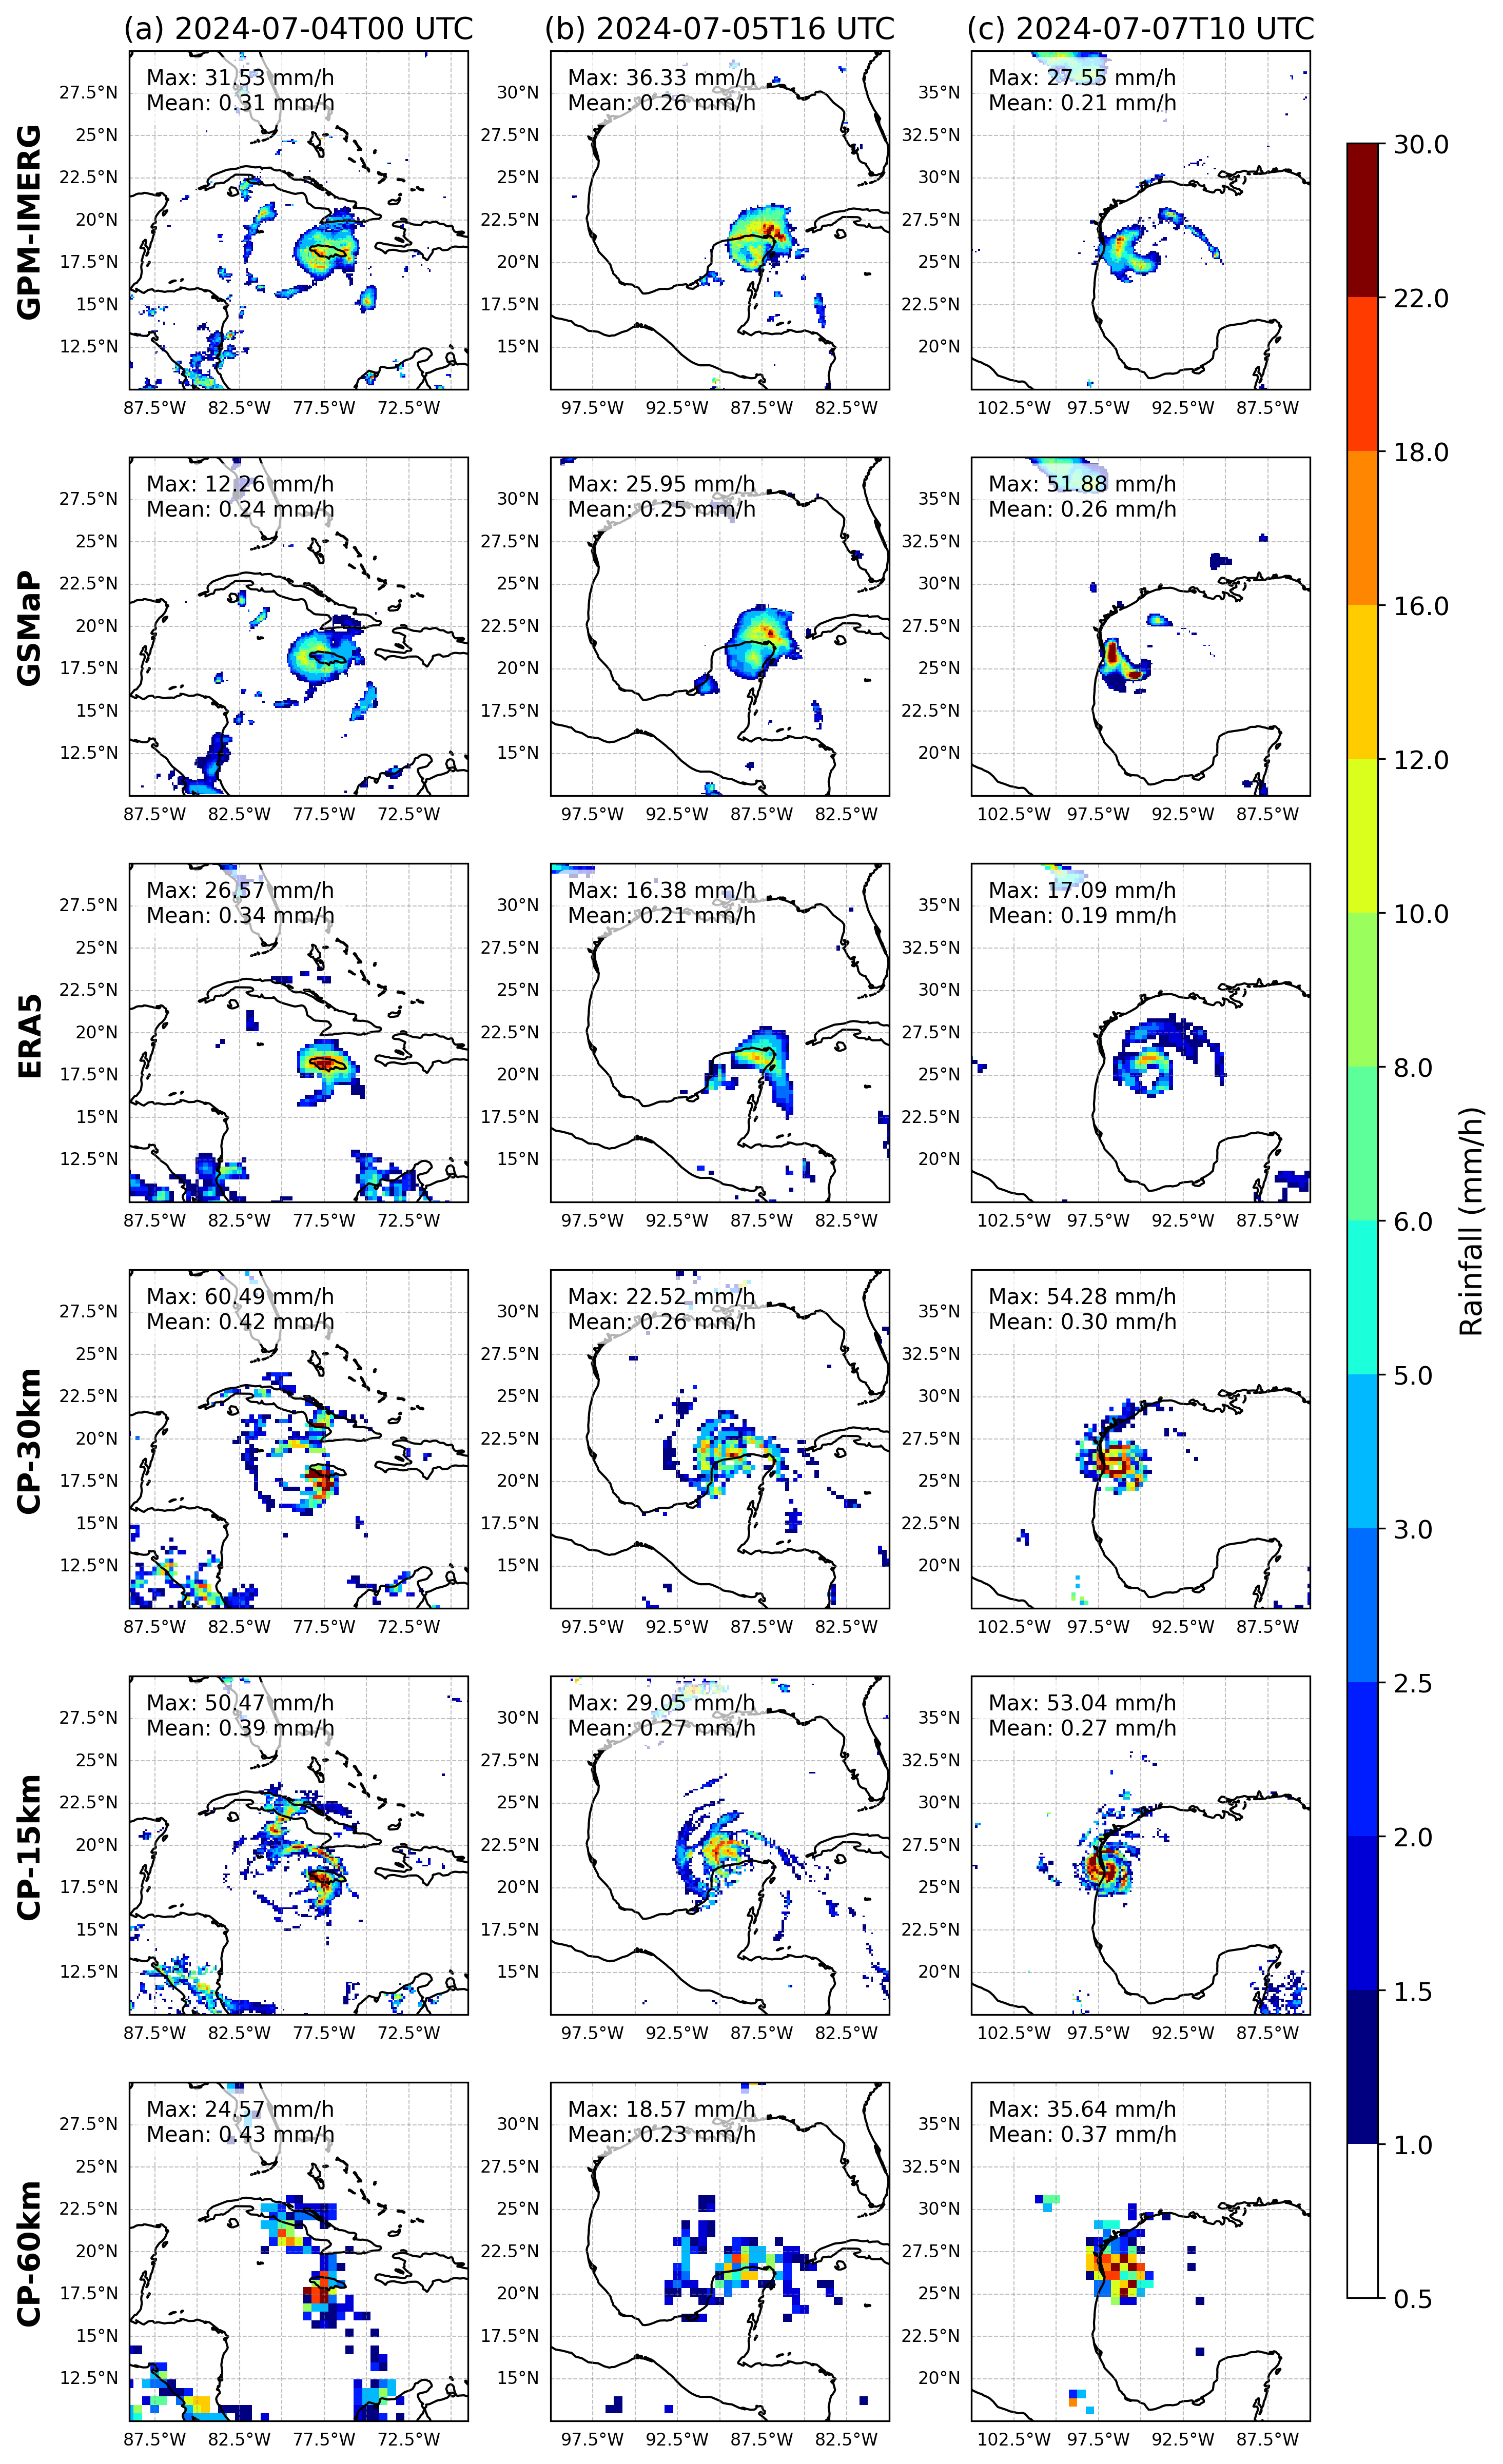
\includegraphics[width=\textwidth]{docs/figuras/chapter5/painel_resolution_rainfall_FINAL.png} 
	\vspace{0.5em}
	Source: Made by the author (2025).  % Fonte abaixo da imagem
	\label{fig:biasgpm2} % Label para referenciar no texto
\end{figure}

The 30 km forecast (CP-30km) performs notably well compared to ERA5 (with 25 km resolution) and GSMaP (4 km resolution), due to its ability to reproduce the spatial characteristics of rainfall seen in GPM-IMERG, especially the arc-shaped rainband observed in panel (a).

A clear gain in spatial detail and rainfall morphology is observed in the 15 km forecast. In particular, the clustering of rainfall and the reproduction of the hurricane's spiral bands stand out, further highlighting the effects of cold pools, features that have also been documented in the literature \cite{sakaeda2023observed}, \cite{freitas2024parameterization}, \cite{haerter2018reconciling}, \cite{feng2015mechanisms}, \cite{vogel2021climatology}. Interestingly, this rainfall clustering effect is also observed in the CP-60km experiment. Despite the loss of detail due to its coarser resolution, it still manages to capture the spiral structure (panel b) and localize regions of intense rainfall (panels a and c). A more detailed investigation (and confirmation) of the role of cold pool parametrization in cloud organization will be left for future work.

Finally, to specifically assess the morphological structure of the clouds, as well as the depth of the cloud tops being formed, the panels in Figure \ref{fig:snapmorph} were created. To isolate the influence of horizontal resolution, Figure \ref{fig:snapmorph2}  was also developed. Once again, these panels were constructed using the same spatial and temporal domains as Figures \ref{fig:snapshot} and \ref{fig:biasgpm2}, but now with cloud-top temperature (i.e., brightness temperature) as the primary variable.

\begin{figure}[!ht]
	\centering
	\caption{Cloud-top brightness temperature snapshots for assessing cloud morphology and vertical structures} % Título acima da figura
	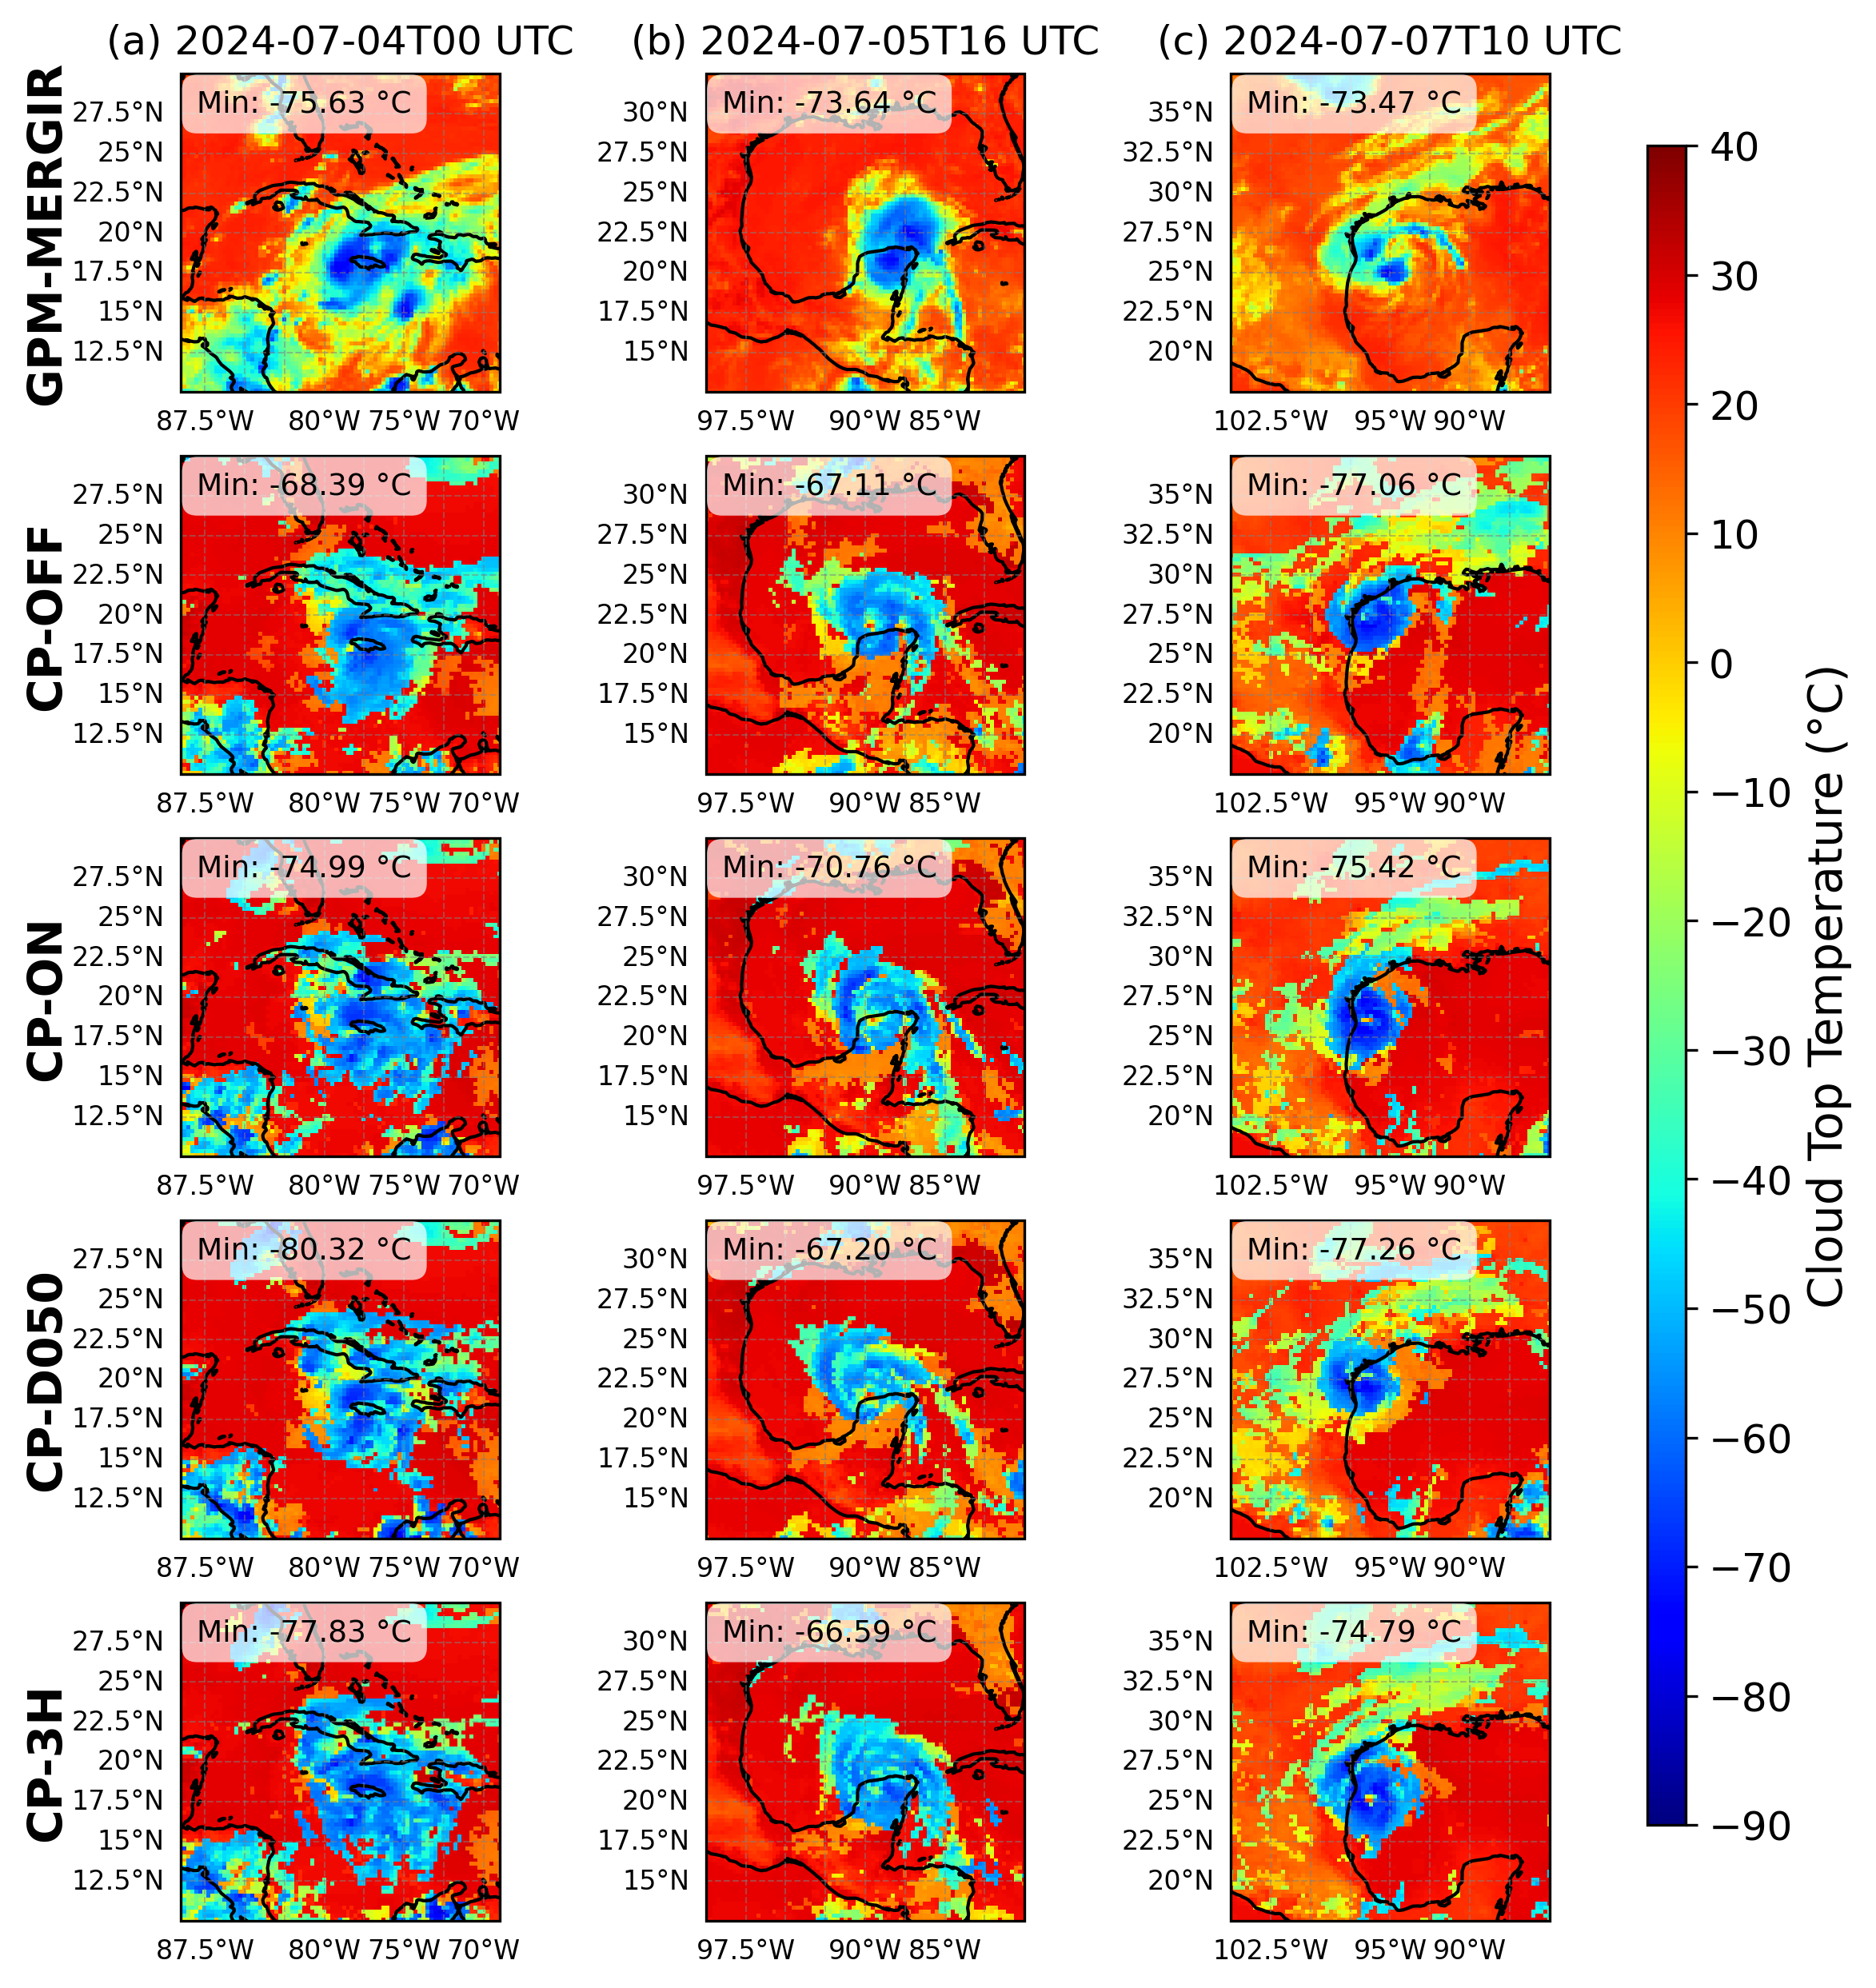
\includegraphics[width=\textwidth]{docs/figuras/chapter5/painel_ctt_selected_experiments_FINAL.png} 
	\vspace{0.5em}
	Source: Made by the author (2025).  % Fonte abaixo da imagem
	\label{fig:snapmorph} % Label para referenciar no texto
\end{figure}

Naturally, the cold pool effect leads to deeper convection, which explains the rainfall values observed in Figures XXX and XXX. It is noteworthy that the cloud-top temperatures in the simulations are very close to those observed, particularly when the cold pool parametrization is active, such as in the CP-ON configuration. The CP-D050 forecast, which has a mass flux profile positioned farther from the surface, produces slightly deeper clouds. This is consistent with its higher cloud base, which results in taller cloud structures overall.

Spatially, cloud coverage in the CP-3H configuration is greater than in the others, due to the duration of the cold pool effect and its ability to continuously generate new cloud populations. In general, the forecasts manage to represent morphological characteristics, such as cloud size and extent, comparable to observations.

\begin{figure}[!ht]
	\centering
	\caption{Effect of horizontal resolution on cloud-top brightness temperature fields} % Título acima da figura
	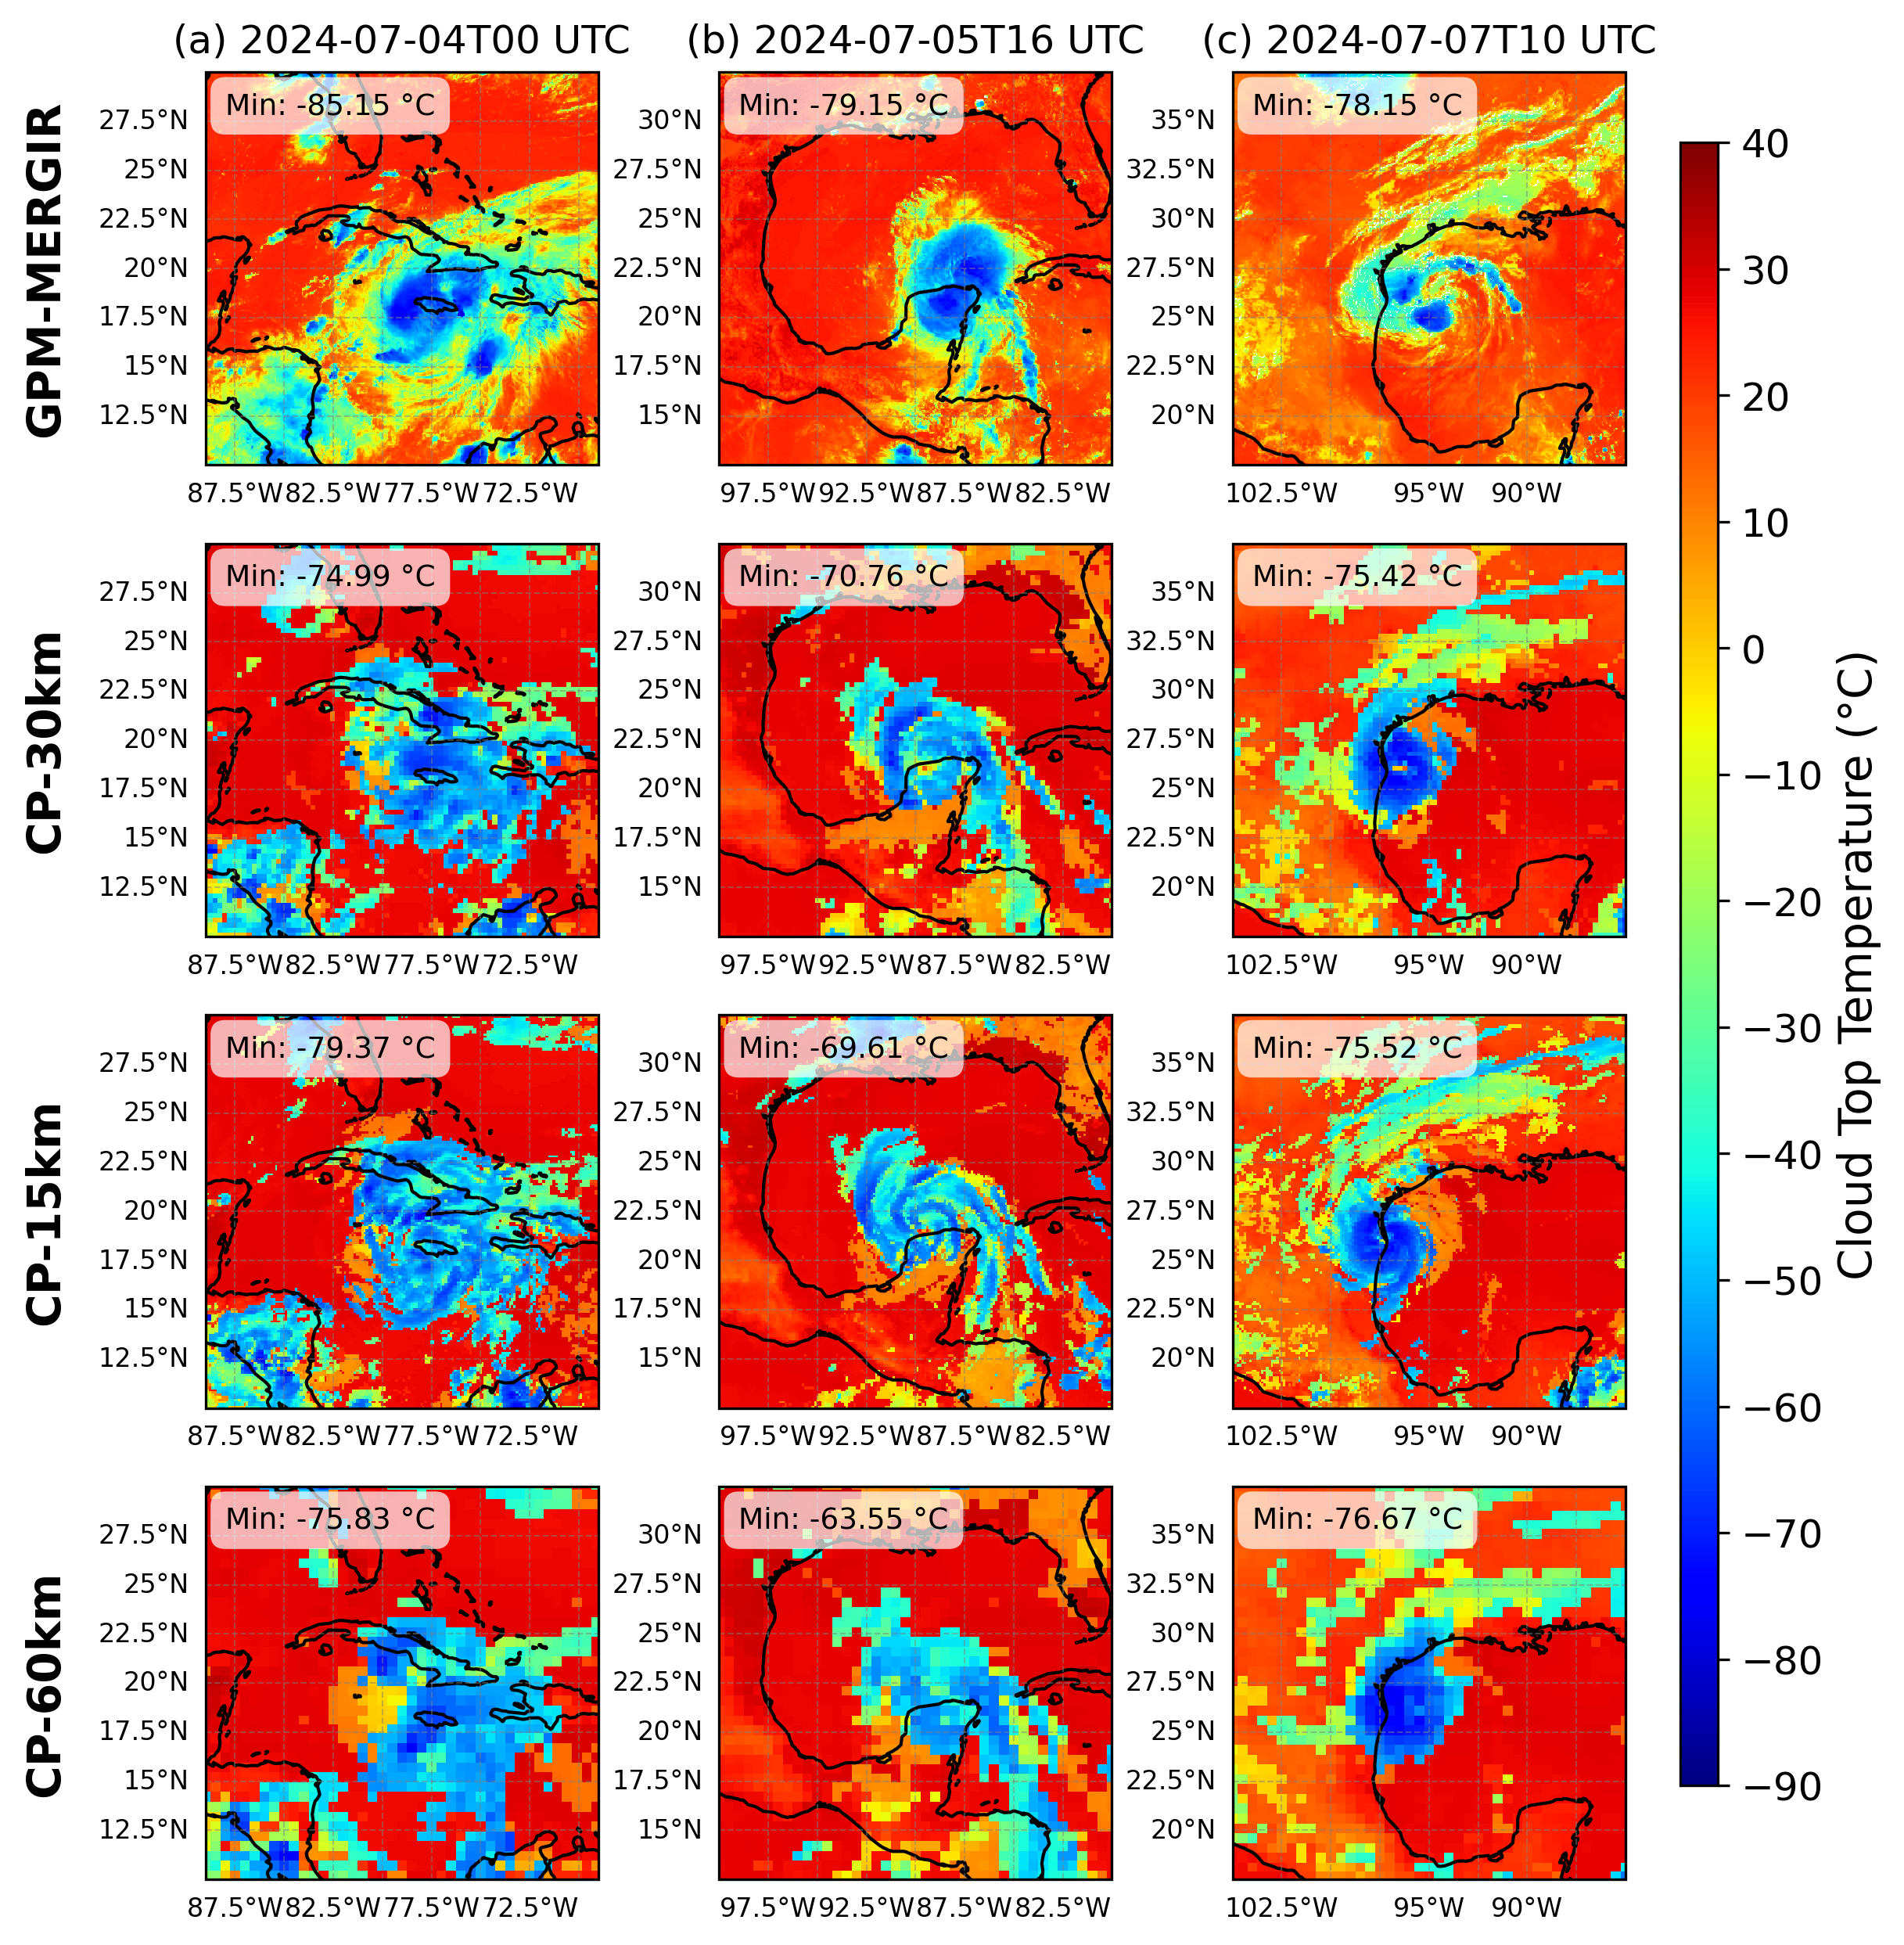
\includegraphics[width=\textwidth]{docs/figuras/chapter5/painel_ctt_native_resolution_FINAL.png} 
	\vspace{0.5em}
	Source: Made by the author (2025).  % Fonte abaixo da imagem
	\label{fig:snapmorph2} % Label para referenciar no texto
\end{figure}

Now, when comparing different resolutions, it becomes clear that the spatial definition of hurricane structure is highly dependent on resolution. At 60 km, the hurricane center becomes nearly indistinguishable, and key structural features, such as the spiral bands, are either poorly resolved or completely absent. In contrast, simulations at 30 km closely resemble those at 15 km in several aspects. Both effectively capture the delineation of the rainbands and the overall spiral organization of the hurricane, with the 15 km forecast naturally providing more detail and sharper gradients. This underscores the significance of horizontal resolution in accurately representing fine-scale convective structures and highlights the threshold at which certain morphological characteristics begin to degrade markedly.

\subsubsection{Rainfall mean and overall distribution}

For this subsection, two types of metrics were employed: Probability Density Functions (PDFs) and Cumulative Distribution Functions (CDFs). As previously mentioned (Section 4), empirical functions are computed, meaning that they are derived directly from the natural distribution of the data. To calculate these functions, a Python script was developed. First, hourly rainfall data over the entire duration of the event (6 days) were gathered. These data were then sorted into thresholds using a logarithmic scale, generating histograms for each experiment, as well as for the GPM-IMERG, ERA5, and GSMaP datasets. Both the forecast and the dataset were at the same horizontal resolution of 30 km. Subsequently, the PDFs and CDFs were computed from these histograms. Note that these distributions are normalized according to the total number of data points. Figure XXX displays the computed PDFs in the first column (A, C, E), and the corresponding CDFs in the second column (B, D, F).

\begin{figure}[!ht]
	\centering
	\caption{Probability density (left) and cumulative distribution functions (right) of hourly rainfall for each experiment and reference dataset} % Título acima da figura
	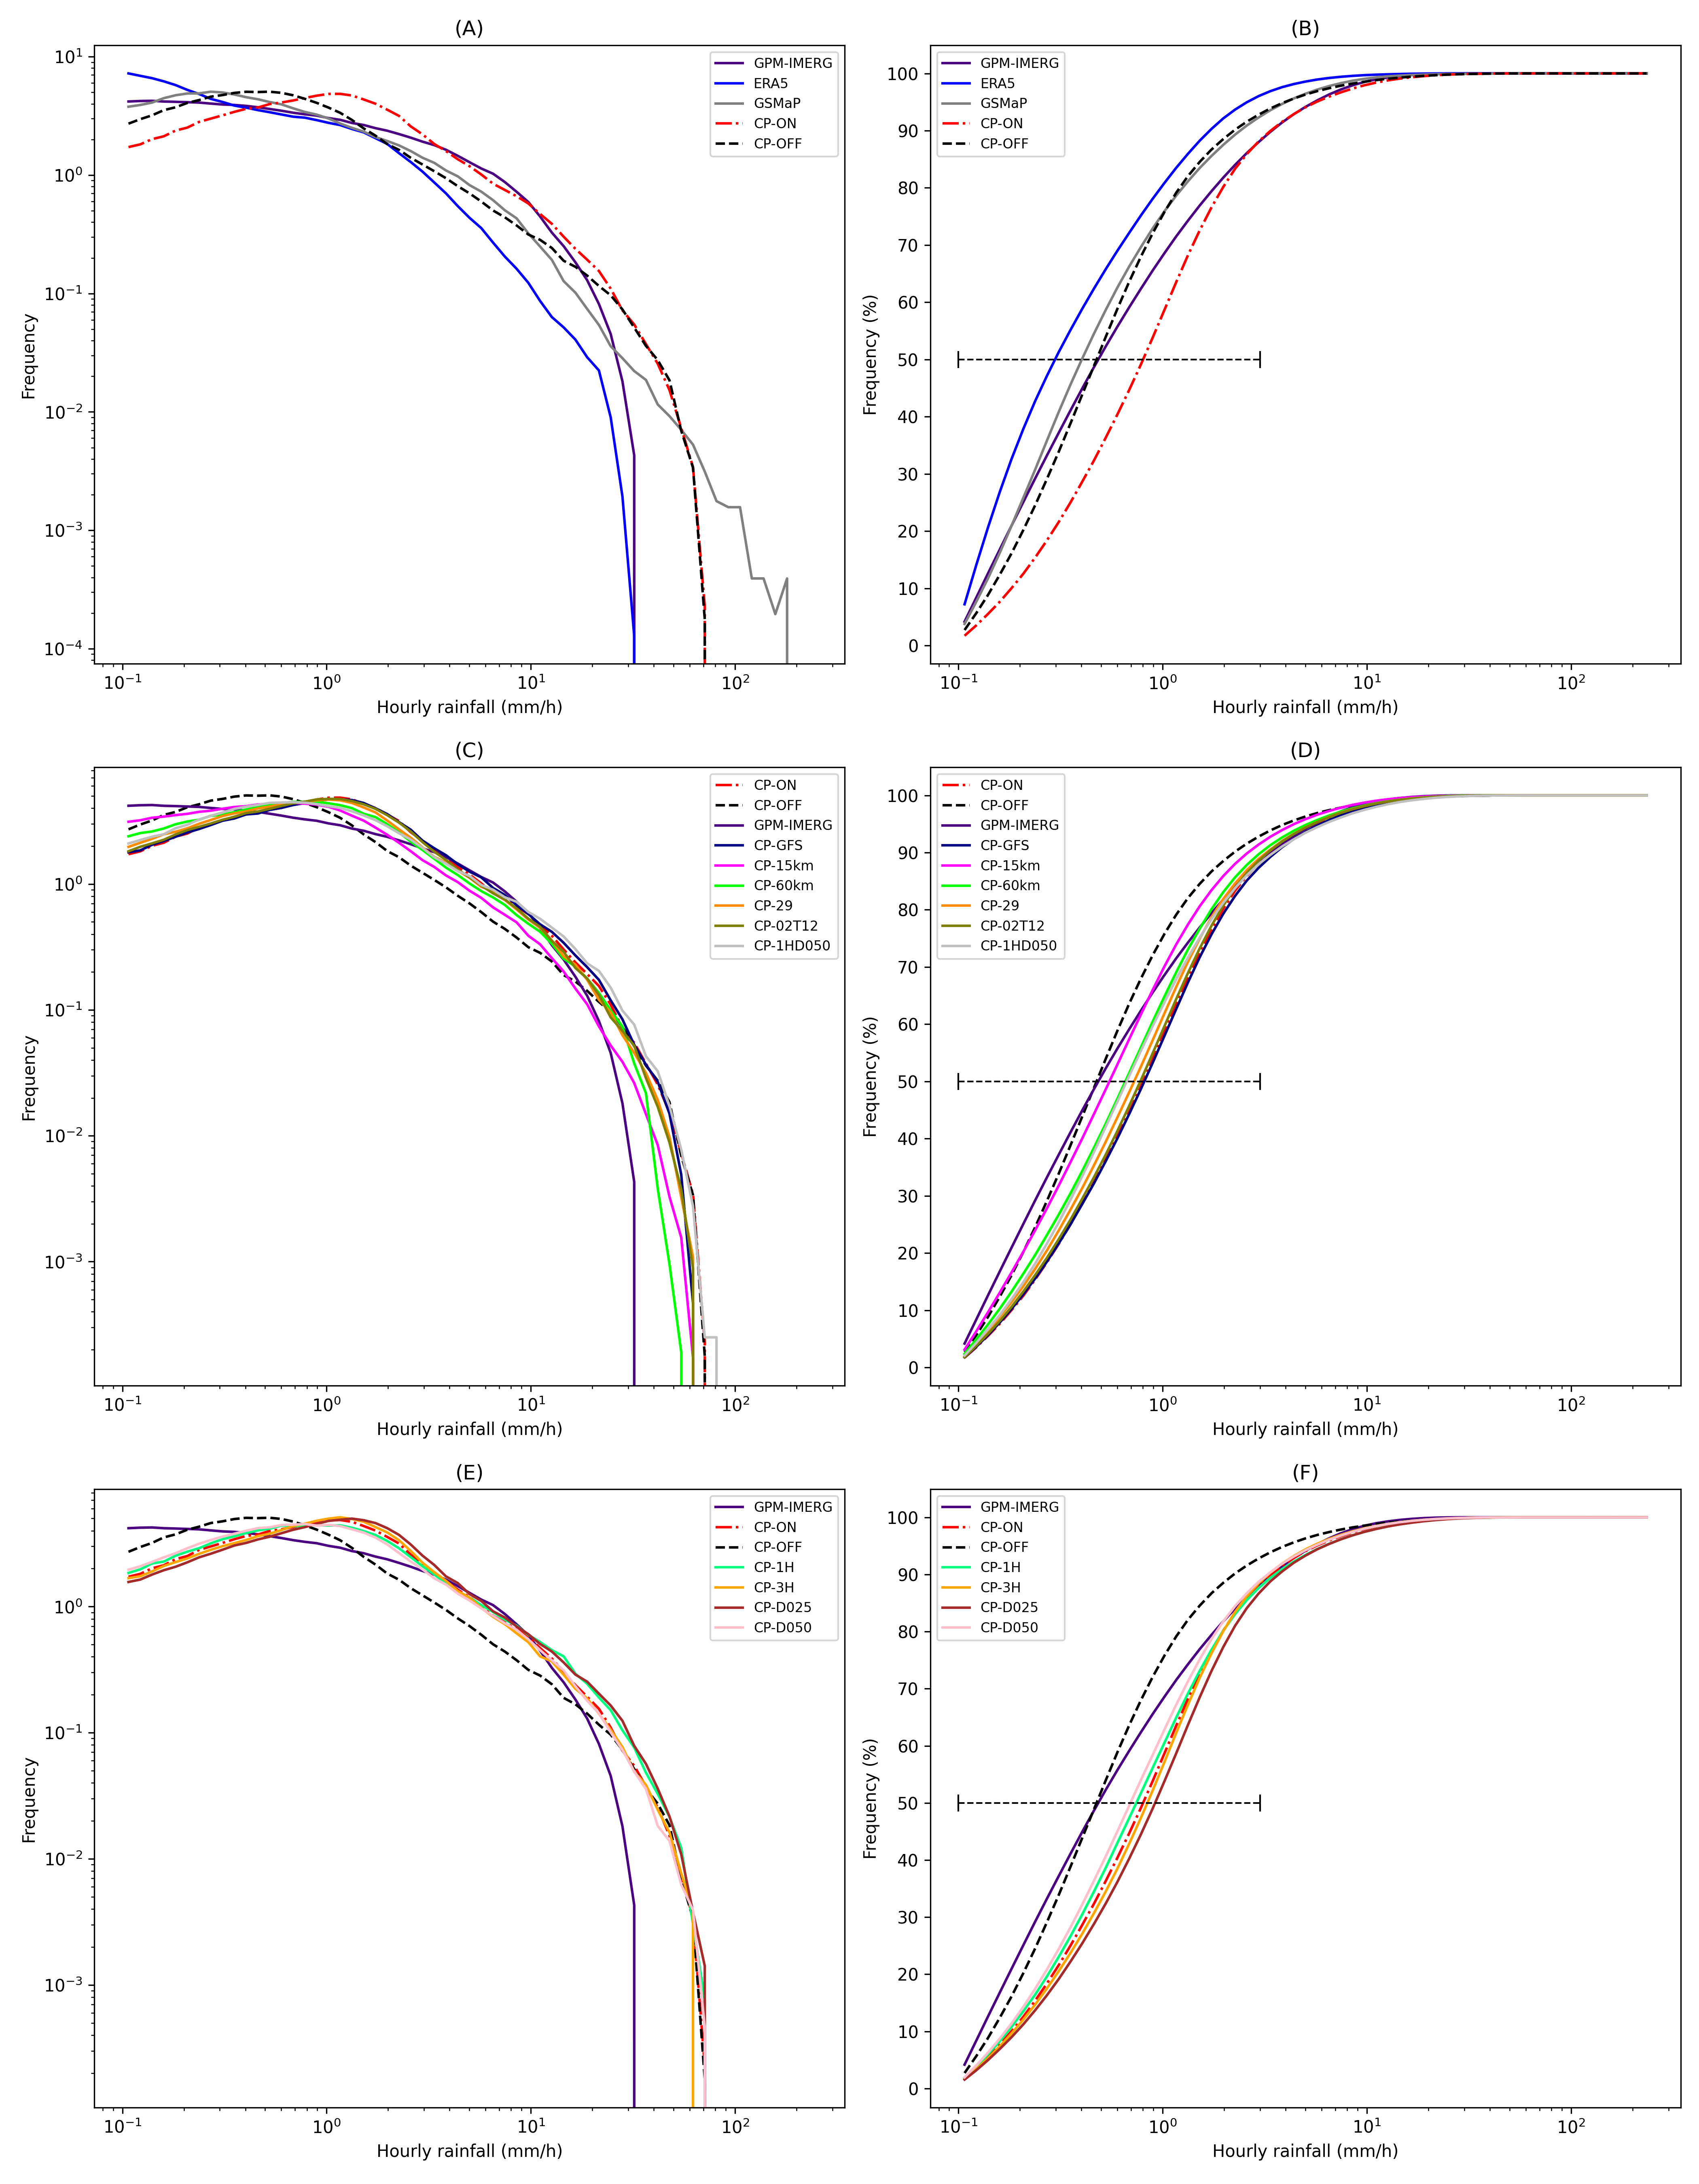
\includegraphics[width=\textwidth]{docs/figuras/chapter5/painel_pdf_cdf_FINAL.png} 
	\vspace{0.5em}
	Source: Made by the author (2025).  % Fonte abaixo da imagem
	\label{fig:probdensity} % Label para referenciar no texto
\end{figure}

In Figure \ref{fig:probdensity} A, ERA5 exhibits a trend similar to GPM-IMERG at lower thresholds but overestimates rainfall in the moderate range (above 1 mm/h), returning to a closer match at higher thresholds, around 20 mm/h. In contrast, GSMaP generally overestimates rainfall at both low and moderate thresholds (up to 20 mm/h), and this overestimation becomes more pronounced at heavy rainfall, exceeding even the MONAN forecasts.

Regarding CP-ON and CP-OFF, both configurations tend to overestimate rainfall at lower thresholds (below 3 mm/h) and at higher extremes (above 10 mm/h), while moderate rainfall shows less bias. At the extremes, both simulations behave similarly; however, CP-ON better matches moderate rainfall values, whereas CP-OFF aligns more closely with the observation at light rainfall values.

This analysis is further supported by Figure \ref{fig:probdensity} B. The horizontal line represents a 50\% frequency (i.e., the median of the distribution). This figure suggests that CP-ON produces a higher average rainfall compared to the other simulations, with CP-OFF showing the closest alignment with GPM-IMERG, and ERA5 producing the lowest values. This behavior is consistent with the cloud morphology analysis, which indicated that CP-ON tends to generate deeper clouds and, consequently, more precipitation. Additionally, for a higher percentage of the sample, near 90\%, CP-ON most closely follows the GPM-IMERG curve, reinforcing its better performance in simulating moderate to heavy rainfall.

Looking at the other sensitivity experiments involving the cold pool parametrization, a similar trend is observed (Figure\ref{fig:probdensity}, C and E). Overall, the parametrization improves the distribution of moderate rainfall, particularly when it is active.

The most significant differences appear in Figure\ref{fig:probdensity} D and F. In Figure Figure\ref{fig:probdensity} D, an improvement in rainfall distribution is evident with increased horizontal resolution (CP-15km), which more closely reproduces the observed GPM-IMERG distribution across all thresholds. It also presents the most accurate average rainfall among all MONAN experiments. On the other hand, panel F demonstrates that certain parameter changes within the cold pool parametrization can degrade the representation of mean rainfall distribution. For example, CP-3H and CP-D025 curves deviate most significantly from the GPM-IMERG mean.

These results suggest that further sensitivity testing, preferably using ensemble approaches, could help better calibrate the forecasted rainfall distributions. Future studies should also include additional hurricane cases to define an optimal cold pool parametrization applicable to various ocean basins.

Finally, one should note that for heavy rainfall thresholds, the curves become indistinguishable, so for the next section we will show a closer look into these thresholds.

\subsubsection{Rainfall extremes}

The following panels represent the CDFs computed for data frequencies above 85\% of each sample (forecasts and datasets), where panels B, D, and F are derived from Figure \ref{fig:probdensity}. In these plots, the vertical purple line indicates the threshold value on the x-axis corresponding to a frequency of 95\%. For GPM-IMERG, this point corresponds to a threshold of 5.5 mm/h, meaning that 95\% of GPM-IMERG data values are equal to or below 5.5 mm/h. On the right side of each graph, the corresponding frequency values for each dataset at this 5.5 mm/h threshold are provided. For example, 98.8\% of ERA5 data exhibit rainfall rates equal to or below 5.5 mm/h; thus, only 1.2\% of ERA5 data exceed this threshold (compared to 5\% from the GPM-IMERG observation).

\begin{figure}[!ht]
	\centering
	\caption{CDFs above the 85th percentile of hourly rainfall, with 95\% threshold comparison across datasets} % Título acima da figura
	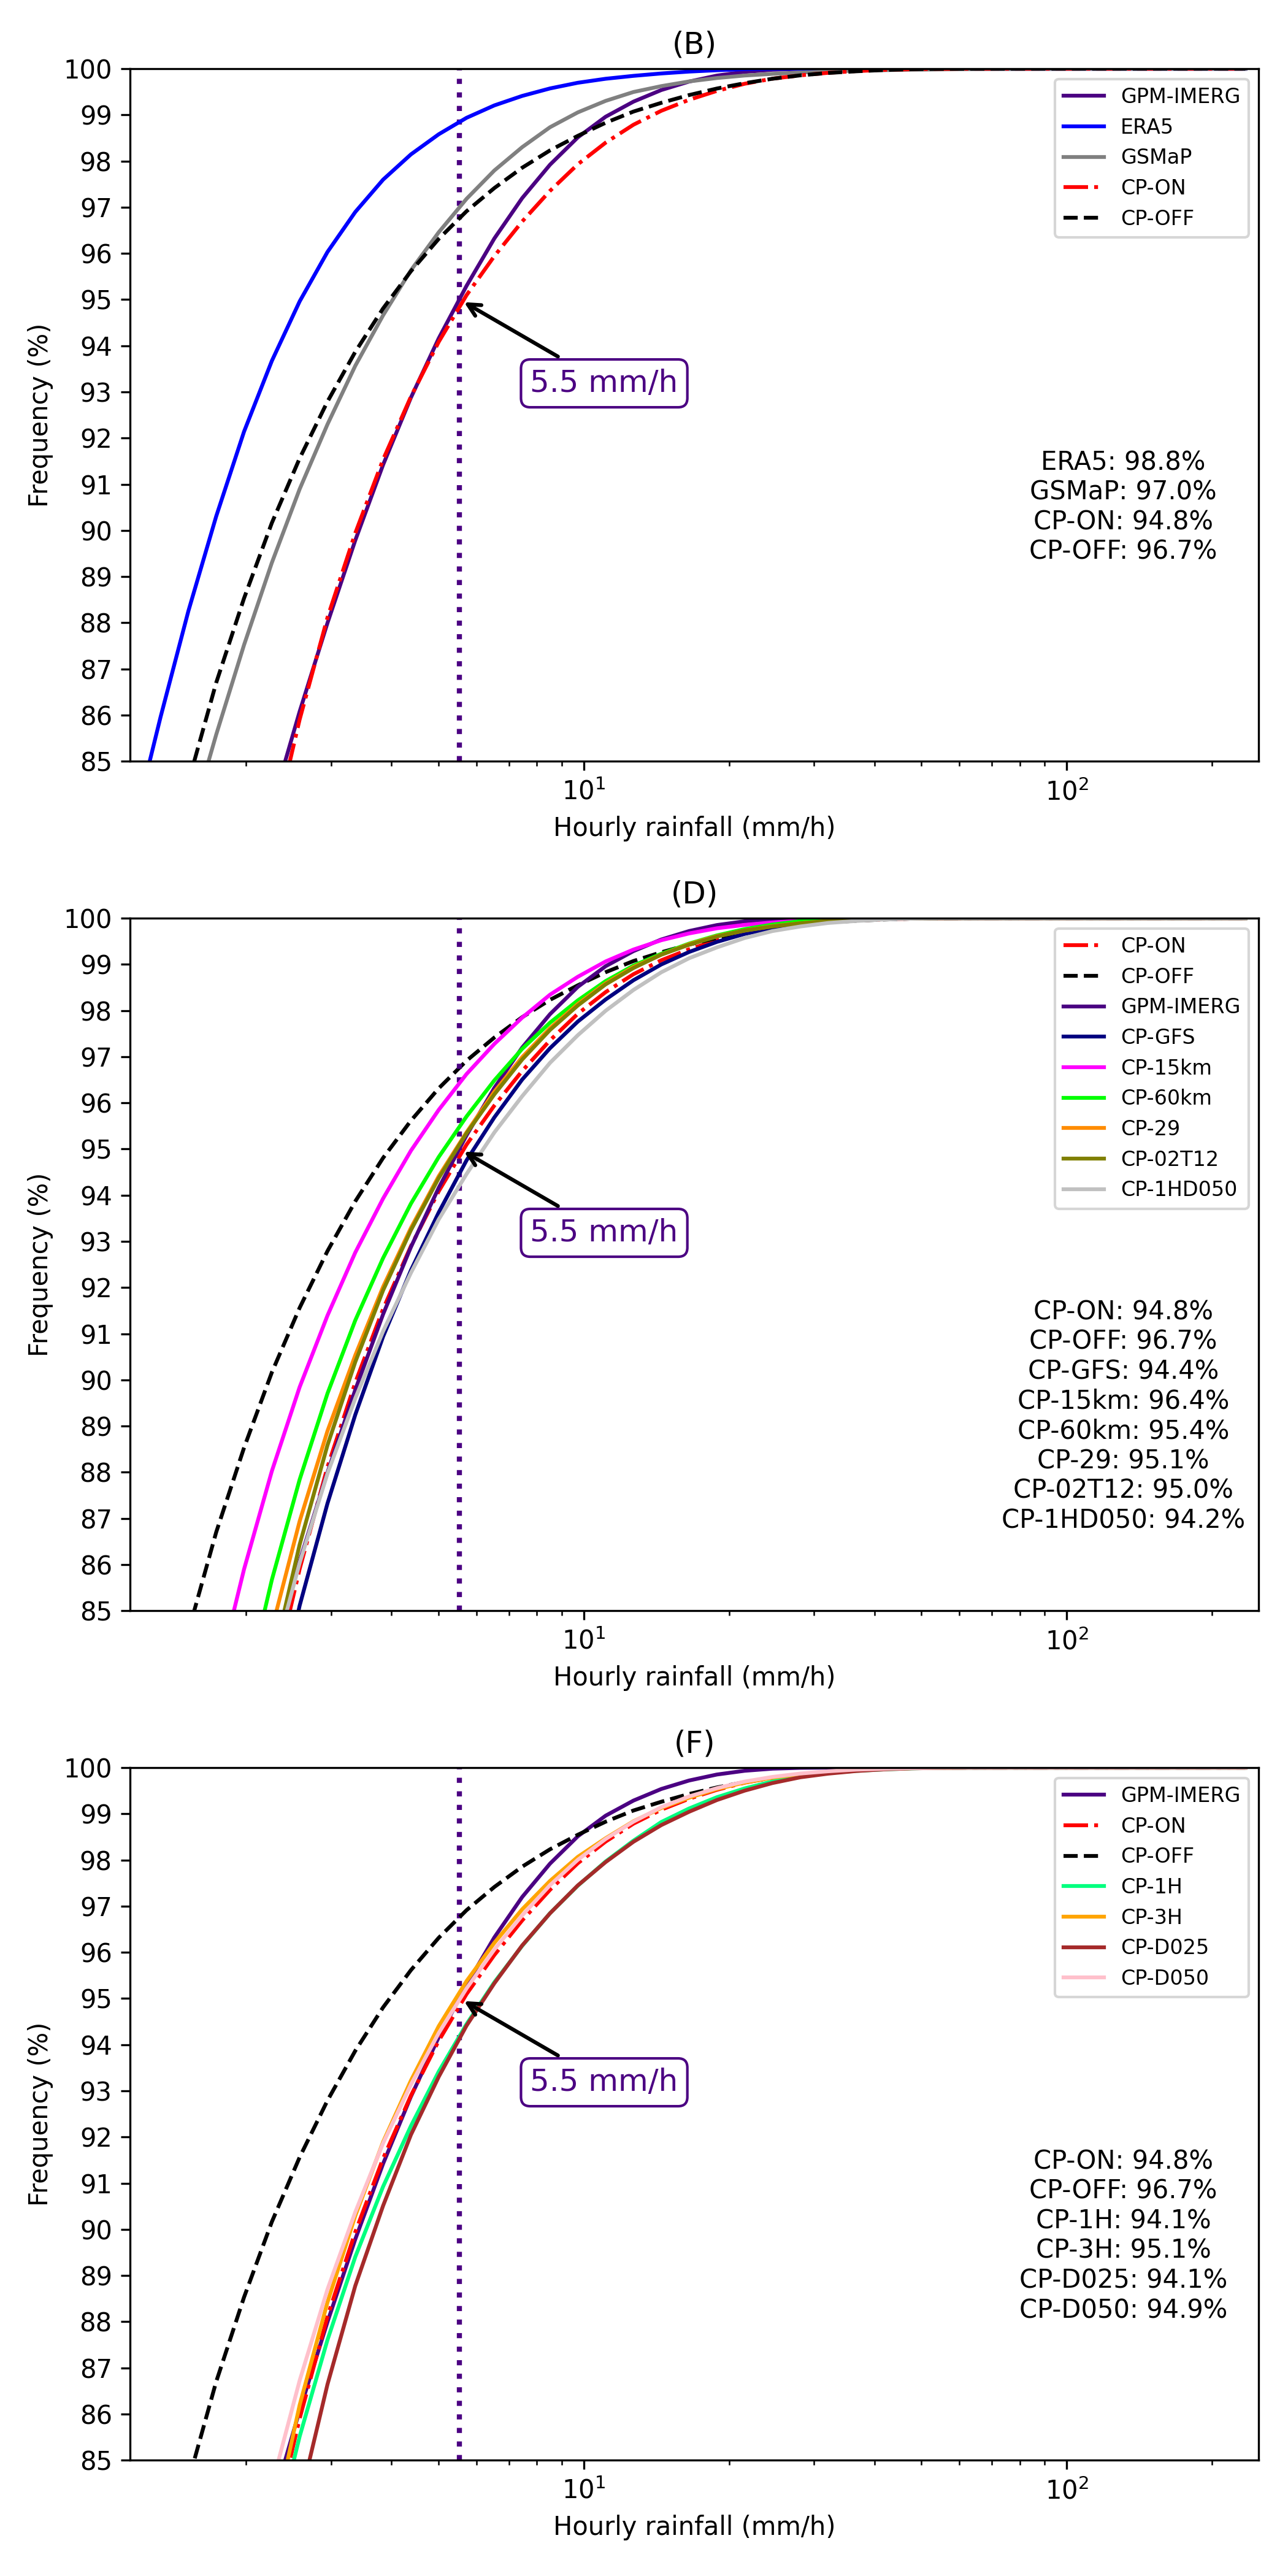
\includegraphics[width=0.7\textwidth]{docs/figuras/chapter5/85_percentile_CDF_FINAL.png} 
	\vspace{0.5em}
	Source: Made by the author (2025).  % Fonte abaixo da imagem
	\label{fig:probdensity2} % Label para referenciar no texto
\end{figure}

Following this logic, the proportion of heavy rainfall produced by each sample becomes clear. CP-ON exhibits the highest heavy rainfall proportion, with approximately 5.2\%, whereas CP-OFF shows only 3.3\%. Additionally, it is worth noting that the percentage of extreme rainfall observed by GSMaP is relatively small, at just 3\%.

Among the sensitivity experiments, the percentage is similar across configurations, with CP-1HD050 yielding 94.2\% of values below 5.5 mm/h (Figure \ref{fig:probdensity2} D), followed by CP-1H and CP-D025 with 94.1\% (Figure \ref{fig:probdensity2} F).

Furthermore, Figure \ref{fig:probdensity3} presents a set of CDFs panels computed using the same spatial and temporal domain as in Figure \ref{fig:probdensity}. That is, each CDF is calculated for the area (latitude and longitude) corresponding to Figure \ref{fig:probdensity} and at specific time steps, displayed in panels A (July 4th 00 UTC), B (July 5th 16 UTC), and C (July 7th 10 UTC). The purpose is to examine how the rainfall distribution behaves when focusing more closely on the hurricane's vicinity.

\begin{figure}[!ht]
	\centering
	\caption{CDFs of hourly rainfall at selected time steps within the hurricane domain} % Título acima da figura
	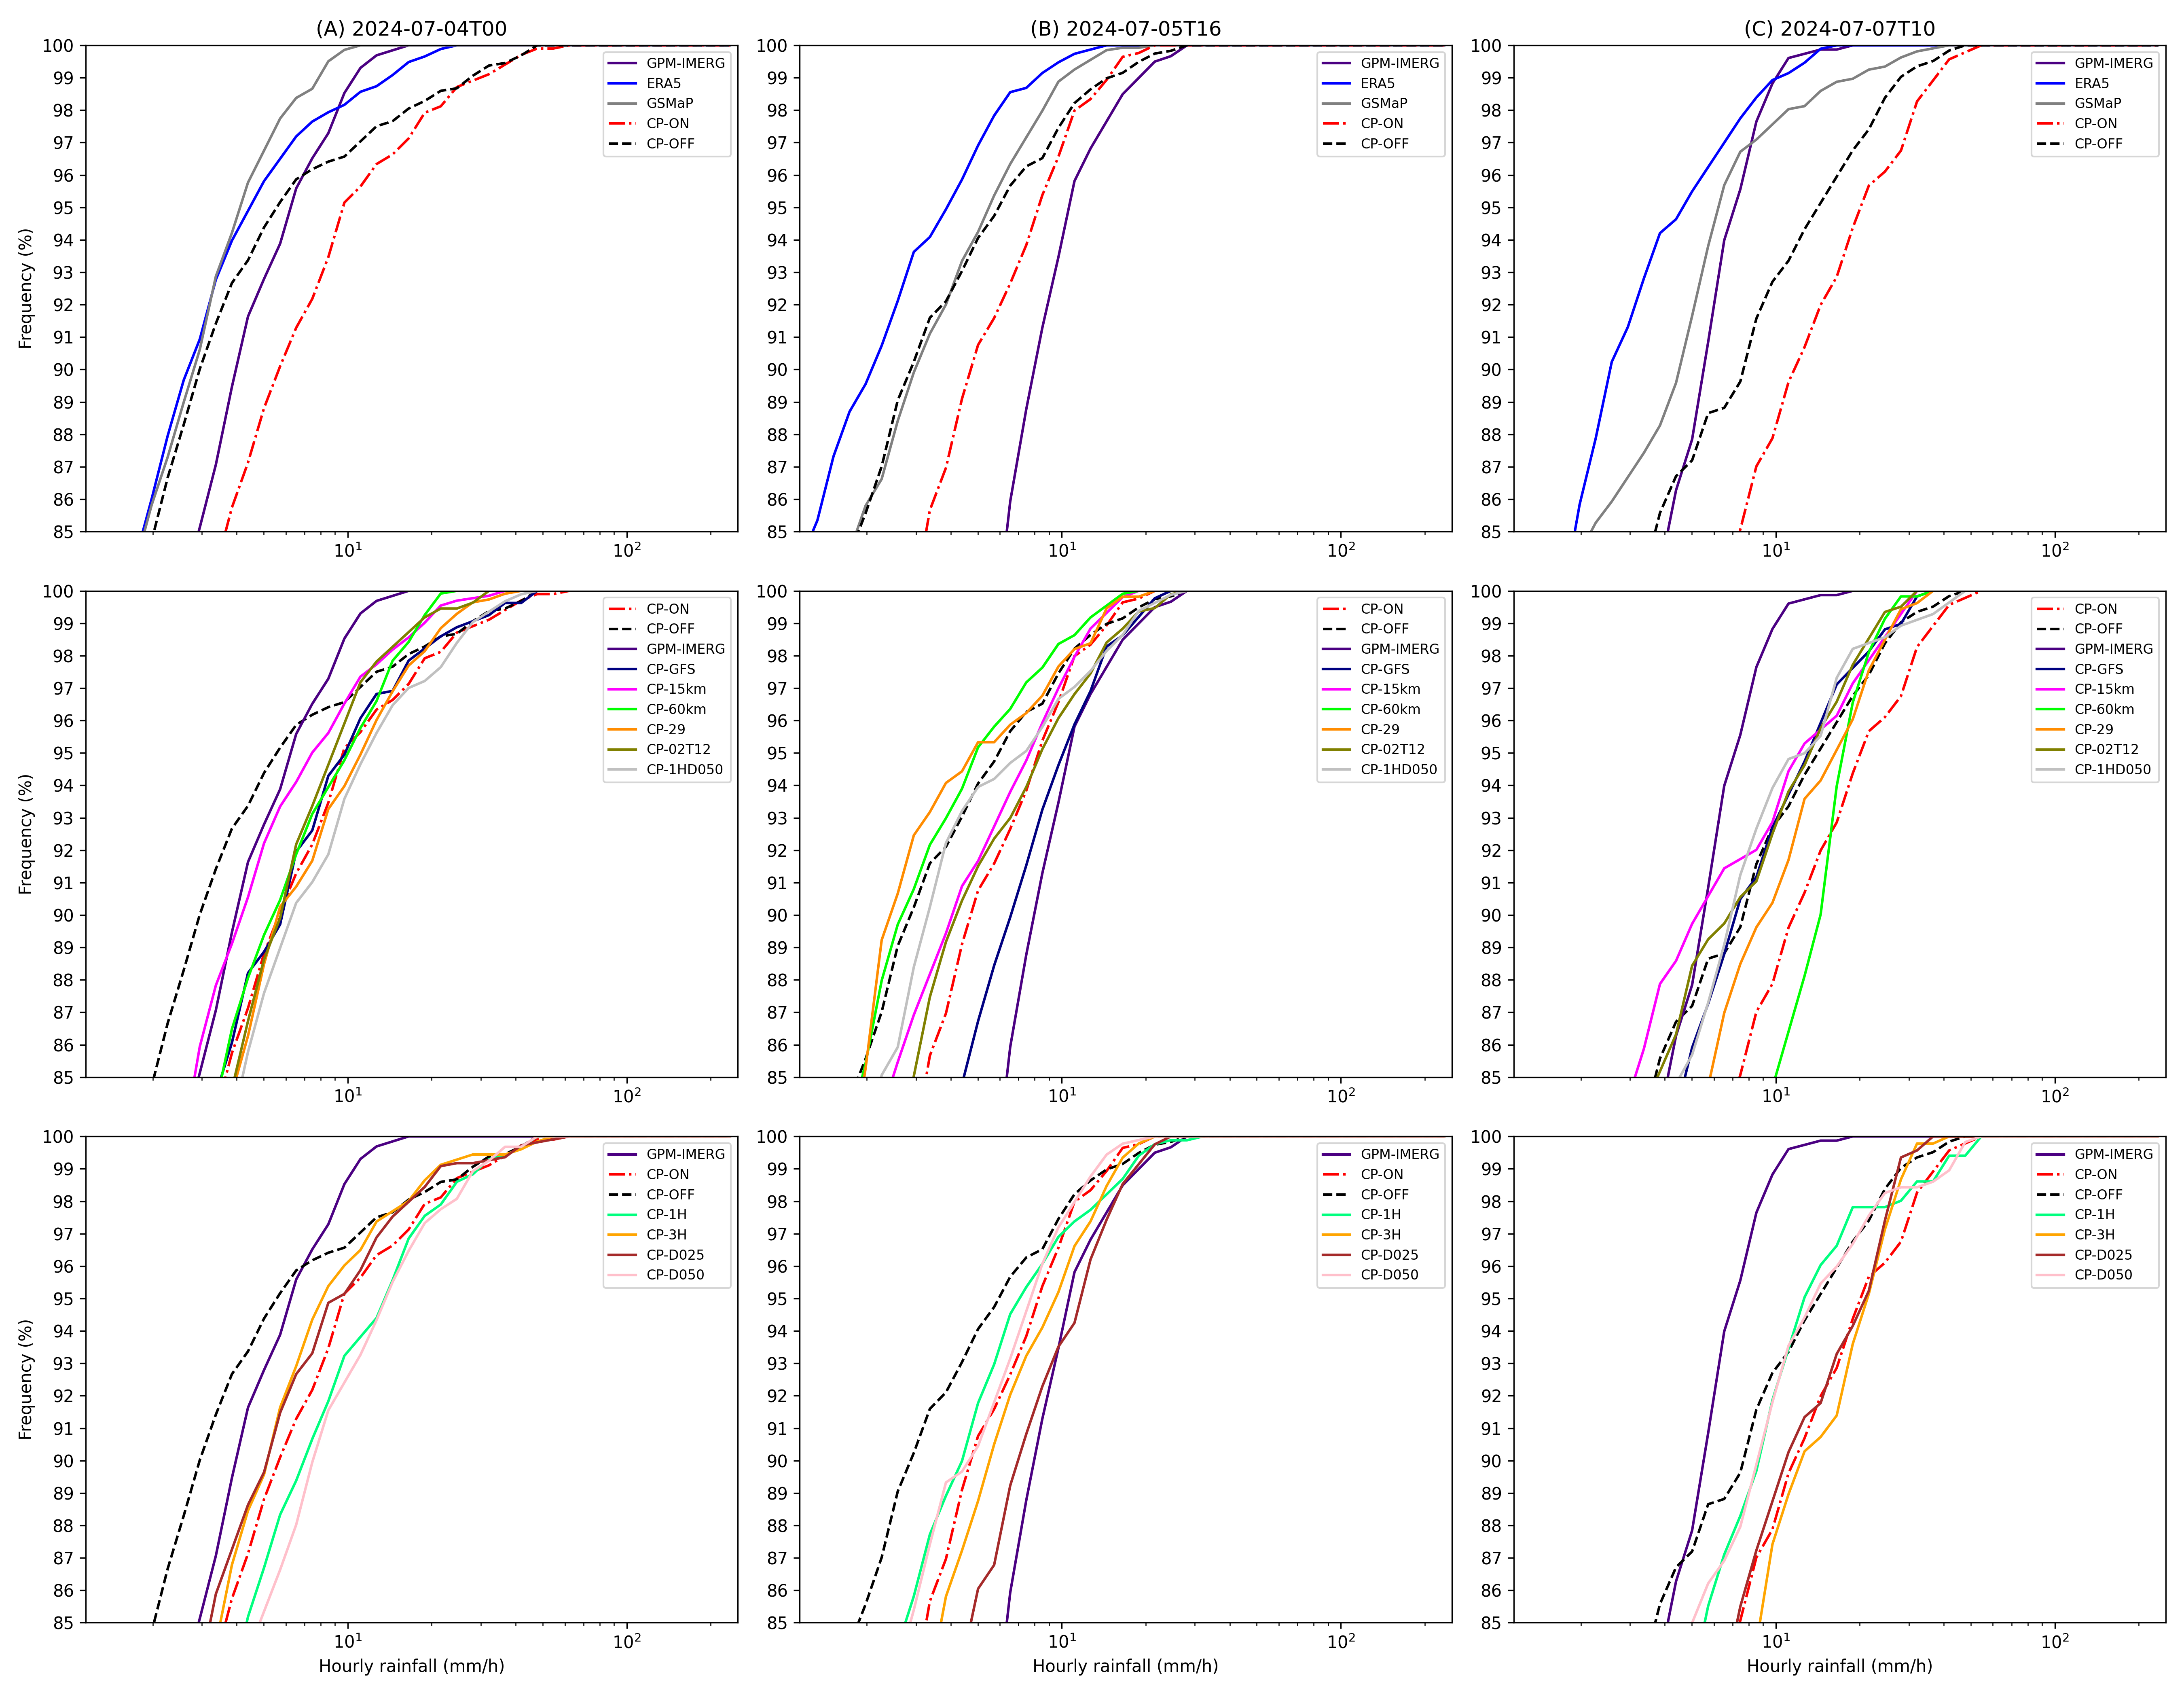
\includegraphics[width=\textwidth]{docs/figuras/chapter5/SNAPSHOTS_percentile_CDF_FINAL.png} 
	\vspace{0.5em}
	Source: Made by the author (2025).  % Fonte abaixo da imagem
	\label{fig:probdensity3} % Label para referenciar no texto
\end{figure}

In the first column (A), corresponding to the moment Beryl reaches its maximum precipitation according to official reports, rainfall is overestimated by the experiments employing the cold pool parameterization, with CP-15km being the closest to the reference. CP-OFF overestimates light rainfall thresholds and significantly overestimates the heavy rainfall range.

After Beryl passes over the Yucatán Peninsula (panel B), most forecasts and datasets tend to overestimate rainfall overall, but they converge better around the heavier rainfall thresholds.

Upon landfall in Texas (panel C), when Beryl re-intensifies to a Category 1 hurricane, there is again a trend of overestimated rainfall. However, this trend is not mirrored by all datasets, and some experiments, such as CP-15km, CP-OFF, and CP-1HD050, show closer agreement at moderate rainfall thresholds.

\subsubsection{MONAN performance at forecasting rainfall}

As this chapter presents a large number of figures and maps, this section aims to concisely summarize the main results by focusing specifically on the eyeball comparison between MONAN and ERA5.

In terms of the Equitable Threat Score (ETS), MONAN shows similar performance to ERA5 overall. The most notable differences occur in the moderate rainfall thresholds, where ERA5 performs higher ETS values.

The Pearson correlation coefficient in the accumulated scene for MONAN averaged 0.45, which is generally considered a moderate correlation, in contrast with ERA5's value of 0.69, which indicates a strong correlation. It is important to highlight that MONAN's correlation deteriorates substantially with increasing forecast lead time. This suggests that if MONAN were initialized more frequently (e.g., with updated initial conditions every day), its correlation values might approach those of ERA5. Despite this degradation, the spatial distribution of extreme rainfall areas is broadly consistent between MONAN and ERA5.

Notably, MONAN can reproduce the convective structures observed by satellite, even with its 30 km horizontal resolution, something that ERA5 fails to capture in certain cases, such as the spiral-shaped rainbands (see case Figure X.X.X).

When analyzing the rainfall distribution and mean values, it was observed that MONAN tends to underestimate rainfall at both lower and higher thresholds, while ERA5 tends to overestimate rainfall at moderate and extreme thresholds. Besides, the mean rainfall in MONAN is slightly overestimated, but on the other hand, in ERA5, it is consistently overestimated.

Finally, in terms of extreme rainfall prediction, MONAN forecasts are closer to the GPM-IMERG reference data, particularly when the convective parameterization is enabled. ERA5, however, tends to significantly overestimate rainfall extremes: for example, 2\% of the sample with extreme rainfall, compared to 5\% observed in GPM-IMERG.

\subsection{Discussion of key outcomes}

a fazer, dale bianca